\documentclass[xcolor=svgnames]{beamer}
\usecolortheme[named=blue]{structure}
\usetheme{theme1}
\usepackage{bm}
\usepackage{amsmath}
\usepackage{amssymb}
\usepackage{amsthm}
\usepackage{graphicx}
\usepackage{xcolor}
\usepackage{mathrsfs}
\usepackage{ragged2e}
\usepackage{calc}
\usepackage{tikz}
\usepackage[T1]{fontenc}
\usepackage[firstinits=true,backend=bibtex,bibstyle=numeric-comp,citestyle=authoryear-comp]{biblatex}
\DeclareCiteCommand{\putCitation}[\mkbibfootnote]
	{\usebibmacro{prenote}}
	{\tiny{
	\printnames[citeauthor]{author}
	\setunit{\addcomma\space}
	\ifentrytype{book}{\printfield{title}}{\printfield[citeield]{shortjournal}}
	(\printfield[citeyear]{year})
	}}
	{\multicitedelim}
	{\usebibmacro{postnote}
}
\DeclareRobustCommand{\abinitio}[0]{\emph{ab initio}}
\DeclareRobustCommand{\Abinitio}[0]{\emph{Ab initio}}
\DeclareRobustCommand{\AbInitio}[0]{\emph{Ab Initio}} % for references
\DeclareRobustCommand{\Schrodinger}[0]{Schr\"{o}dinger}
\DeclareRobustCommand{\Sim}[0]{$\sim$}
\DeclareRobustCommand{\PESs}[0]{PES\,s}
\DeclareRobustCommand{\mc}[1]{\mathcal{#1}}
\DeclareRobustCommand{\mbf}[1]{{\boldsymbol {#1}}}
\addbibresource{masterReferences.bib}
\addtobeamertemplate{frame begin}{}{\justifying}
\title{Quantum Virial Coefficients via Path Integral Monte Carlo: Theory and Development of Novel Algorithms}
\author{PhD dissertation defense by: Ramachandran Subramanian}
\institute[UB]{
    Committee: Prof. David A. Kofke (Chair),\\
Prof. Jeffrey R. Errington, Prof. Johannes Hachmann, Dr. Andrew J. Schultz
}
\date{May 9, 2016}


\AtBeginSection[]
{
\begin{frame}
\frametitle{Overview}
\tableofcontents[currentsection]
\end{frame}
}


\begin{document}
	{
	\setbeamertemplate{headline}{}
	\setbeamertemplate{footline}{}
	\begin{frame}
		\titlepage
	\end{frame}
	}
	
	\iffalse
	\begin{frame}
		\frametitle{Overview}
		\tableofcontents
	\end{frame}
	\fi
	
	\section{Introduction}
	\subsection{Viral coefficients}
		\begin{frame}
			\frametitle{Virial equation of state (VEOS)}
                \begin{block}{}
                    \color{blue}{
                    \begin{equation*}
                        \frac{P}{\rho kT} = 1 + B_2(T) \rho + B_3(T) \rho^2 + \ldots
                    \end{equation*}}
                \end{block}
			\begin{itemize}
				\justifying
				\item $B_n$ - $n^{th}$ order virial coefficient represents the effect of interaction of $n$ molecules.
				\item Depends only on temperature.
				\item Works well for systems with low density (typically gases).
			\end{itemize}
		\end{frame}

        \begin{frame}
			\frametitle{Expressions for the virial coefficients}
			\begin{itemize}
				\justifying
				\item Second and third order virial coefficients are given by:
                \begin{equation}
                    \begin{aligned}
                        B_2(T) &= -\frac{1}{2} \displaystyle\int d1 ~ f(0,1)\\
                        B_3(T) &= -\frac{1}{3} \displaystyle\int \int d1~d2~f(0,1)~f(0,2)~f(1,2)
                    \end{aligned}
                \end{equation}
                where $f(0,1) = \Big( \exp \big[ -\beta U_2(\mbf{r}) \big] - 1 \Big) $ and indices `1' and `2' denote the position and orientational degrees of freedom of molecules 1 and 2, respectively, with respect to molecule `0' at the origin.
            \item The number of such integrals to be summed\putCitation{Hansen} is: 3 for B$_4$, 10 for B$_5$, 56 for B$_6$, 468 for B$_7$.
			\end{itemize}
		\end{frame}

		\begin{frame}
            \frametitle{Main uses:}
			\begin{itemize}
				\justifying
				\item To compute other thermodynamic properties like the joules-thomson coefficient, critical point etc.
                \item To rank different potential models by comparing their virial coefficients to experimental results
				\begin{figure}
				\centering
				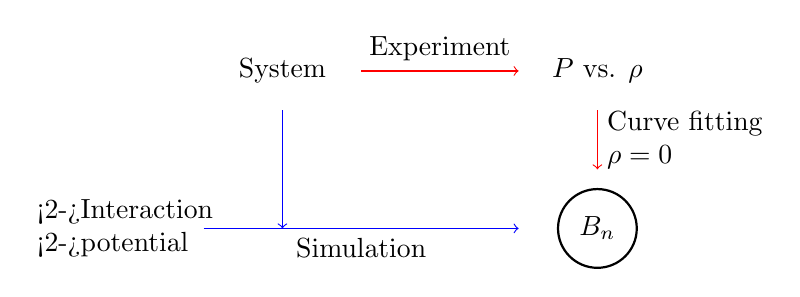
\begin{tikzpicture}
				\node at (-2,3) {System};
				\draw[->,red] (-1,3) -- (1,3);
				\node[above] at (0,3) {Experiment};
				\node at (2,3) {$P$ vs. $\rho$};
				\draw[->,red] (2,2.5) --(2,2.125) node[align=left,right,black]{Curve fitting\\ $\rho = 0$ } -- (2,1.75);
				\node at (2,1) {$B_n$};
				\draw[thick] (2,1) circle [radius=0.5];
				\node[align=left] at (-4,1) {\alert<2->{Interaction}\\ \alert<2->{potential}};
				\draw[->,blue] (-3,1) -- (-1,1) node[below,black] {Simulation} -- (1,1);
				\draw[->,blue] (-2,2.5) -- (-2,1);
				\end{tikzpicture}
				\end{figure}
            \item \visible<2->{To systematically tune and improve potentials as a result.}
			\end{itemize}
		\end{frame}
		
		\begin{frame}
			\frametitle{Empirical potential models}
			\begin{itemize}
				\justifying
				\item Usually functions fitted to experimental data of bulk property measurement.
				\item Represent the net effect of a variety of phenomenon taking place including 2 body interactions, multi-body interactions, nuclear quantum effects etc.
				\item As a result, fail to accurately represent interaction potential.
				\item Interaction potentials that better represent condensed (high density) phase fail to predict accurate virial coefficients for the gas (low density) phase.
			\end{itemize}
		\end{frame}
		
		\begin{frame}
			\frametitle{Example - different empirical models of water}
            \begin{itemize}
                \item Importance of the accuracy of interaction potential\putCitation{Benjamin2007}:
            \end{itemize}
            \begin{figure}
            \centering
            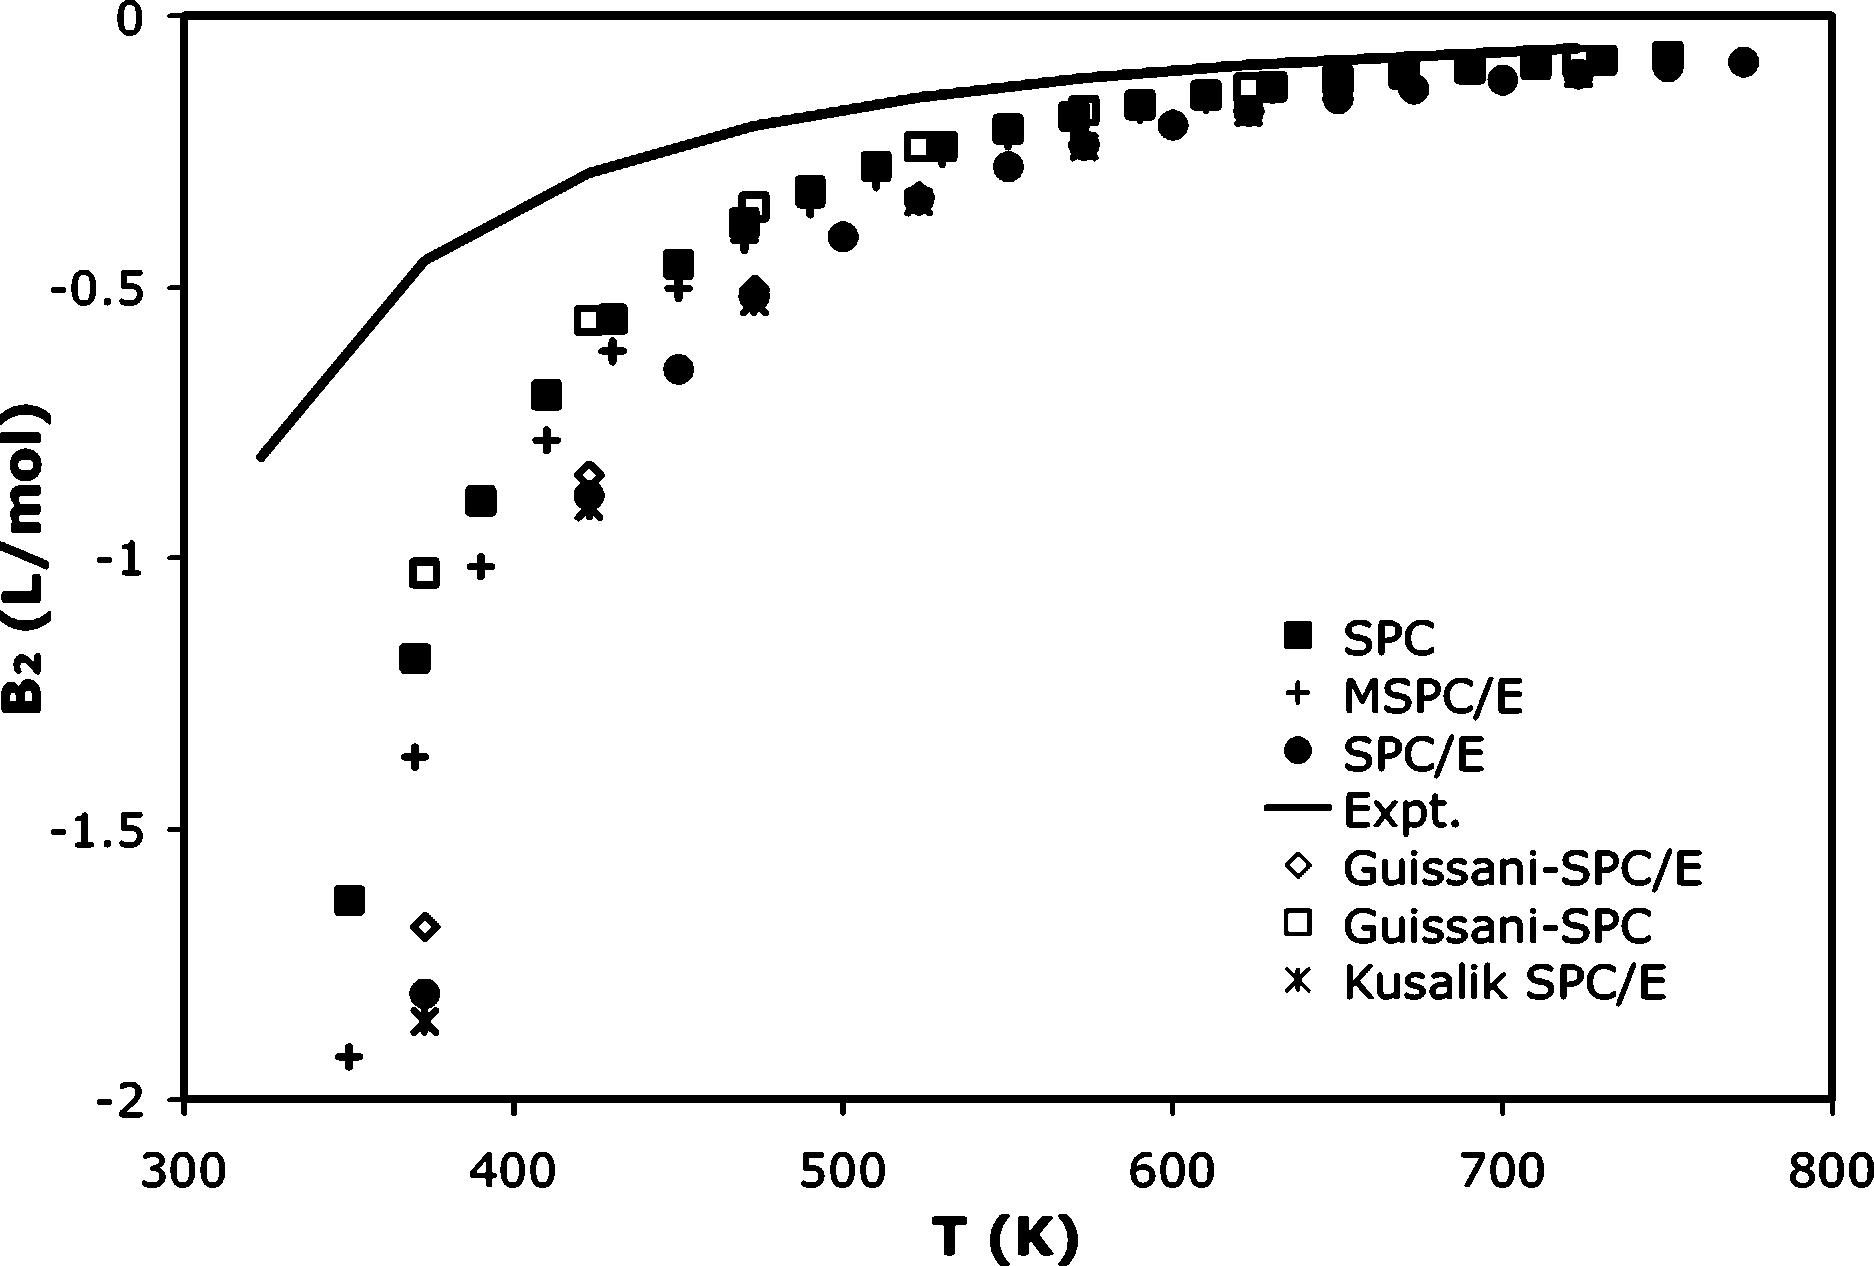
\includegraphics[scale=0.08,keepaspectratio]{ben2a.png}
            \end{figure}
		\end{frame}
    \subsection{\Abinitio{} potentials}
        \begin{frame}
        \frametitle{\Abinitio{} potential models}
            \begin{itemize}
                \item Fundamentally different from empirical models as they focus only on two or three molecules at a time
                \item Solve for the interaction energies starting with the \Schrodinger{} equation and involve many approximations:
                \begin{equation*}
                    \begin{aligned}
                        \mc{H}~\Psi &= E~\Psi, \\
                        \mc{H} &= \mc{T}_e + \mc{T}_N + \mc{V}_{ee} + \mc{V}_{eN} + \mc{V}_{NN}
                    \end{aligned}
                \end{equation*}
                \item Account for electronic structure using different levels of theory and different basis sets
                \item We use potentials fitted to \abinitio{} data rather than compute it on-the-fly (expensive)
            \end{itemize}
            \end{frame}

        \begin{frame}
            \frametitle{Nuclear quantum effects}
            \begin{itemize}
                \justifying
                \item Consequence of uncertainty in the positions of atoms at low temperatures (Zero-point vibrational energy).
                \item Have to be explicitly included in virial coefficient calculations as they are ignored in the development of \abinitio{} potentials.
                \item Semi-classical routes to include quantum effects:
                    \begin{enumerate}
                        \item Computing first order quantum corrections.
                        \item Using an effective potential like the Quadratic Feynman-Hibbs\putCitation{Feynman}.
                    \end{enumerate}
                \item Quantum route: path integral Monte Carlo (PIMC) (will be explained in detail later).
            \end{itemize}
        \end{frame}
        \begin{frame}
            \frametitle{Classification of virial coefficients}
            \begin{itemize}
                \item Different levels of ``quantumness'', using $B_2$ as an example:
            \end{itemize}
            \begin{figure}
            \centering
            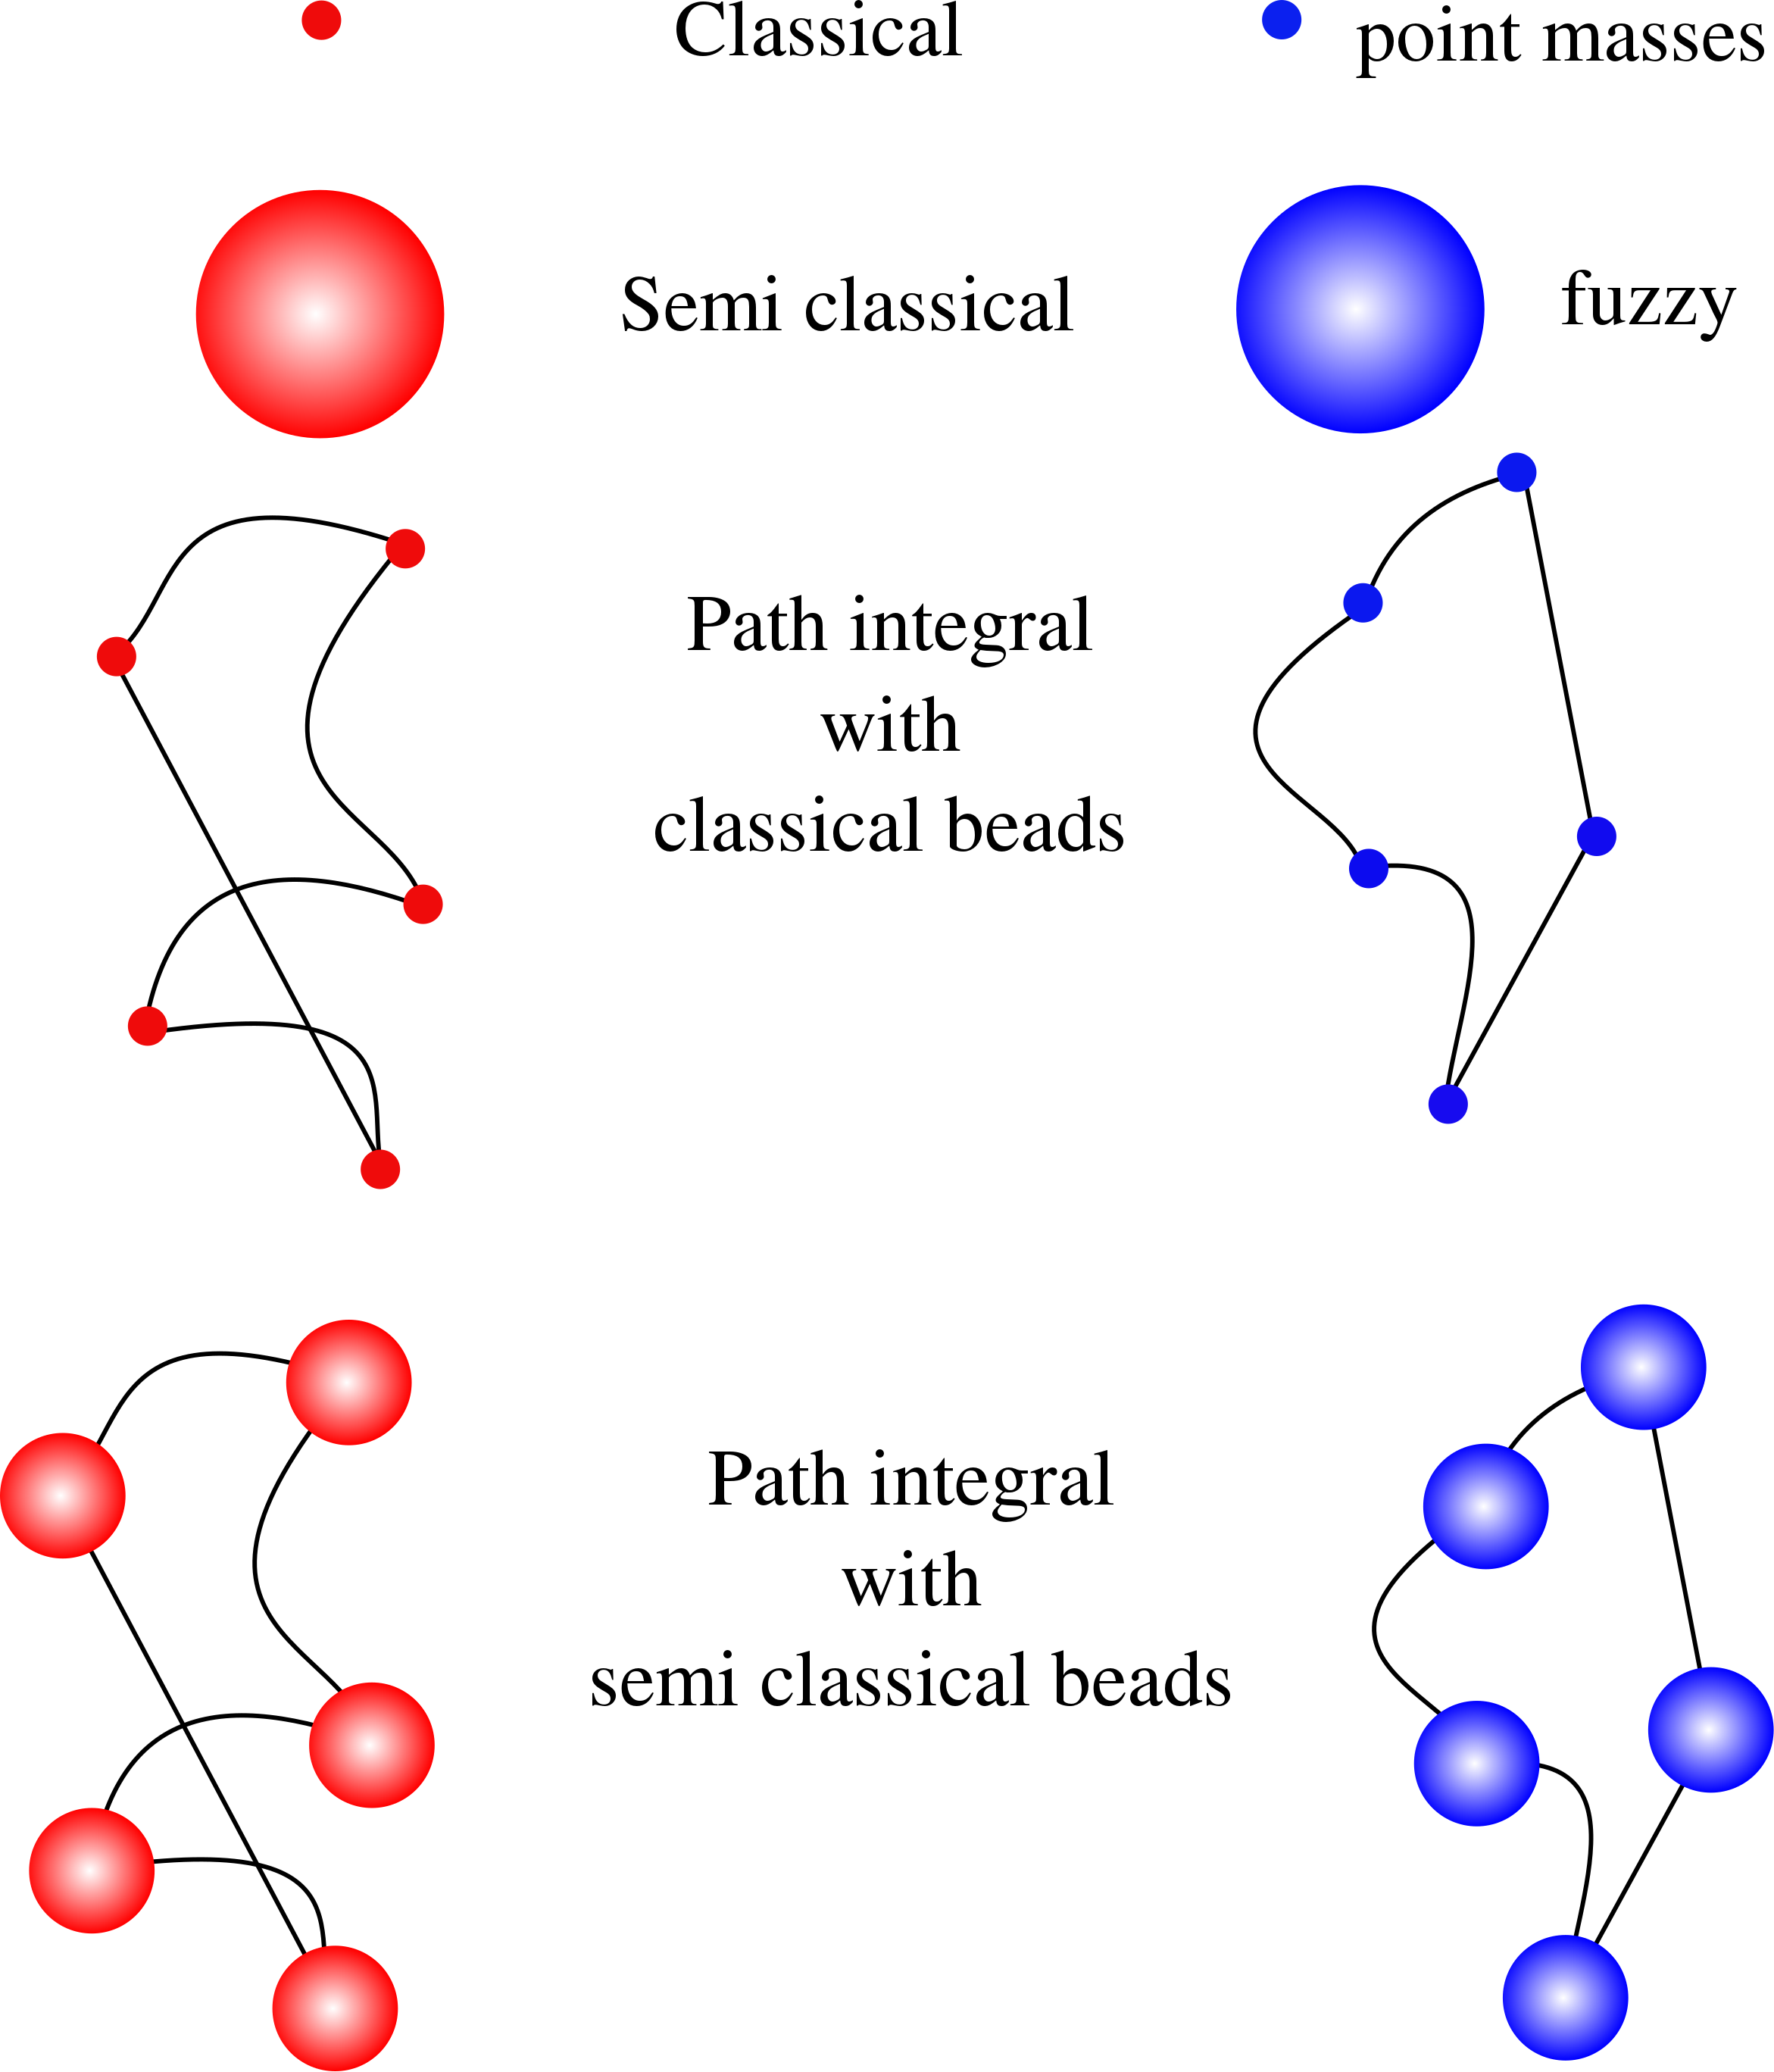
\includegraphics[scale=0.05,keepaspectratio]{quantumLevels.png}
            \end{figure}
        \end{frame}
        \begin{frame}
            \frametitle{Nuclear quantum effects}
            \begin{itemize}
                \item Importance of nuclear quantum effects\putCitation{Shaul2012}
            \end{itemize}
            \begin{figure}
            \centering
            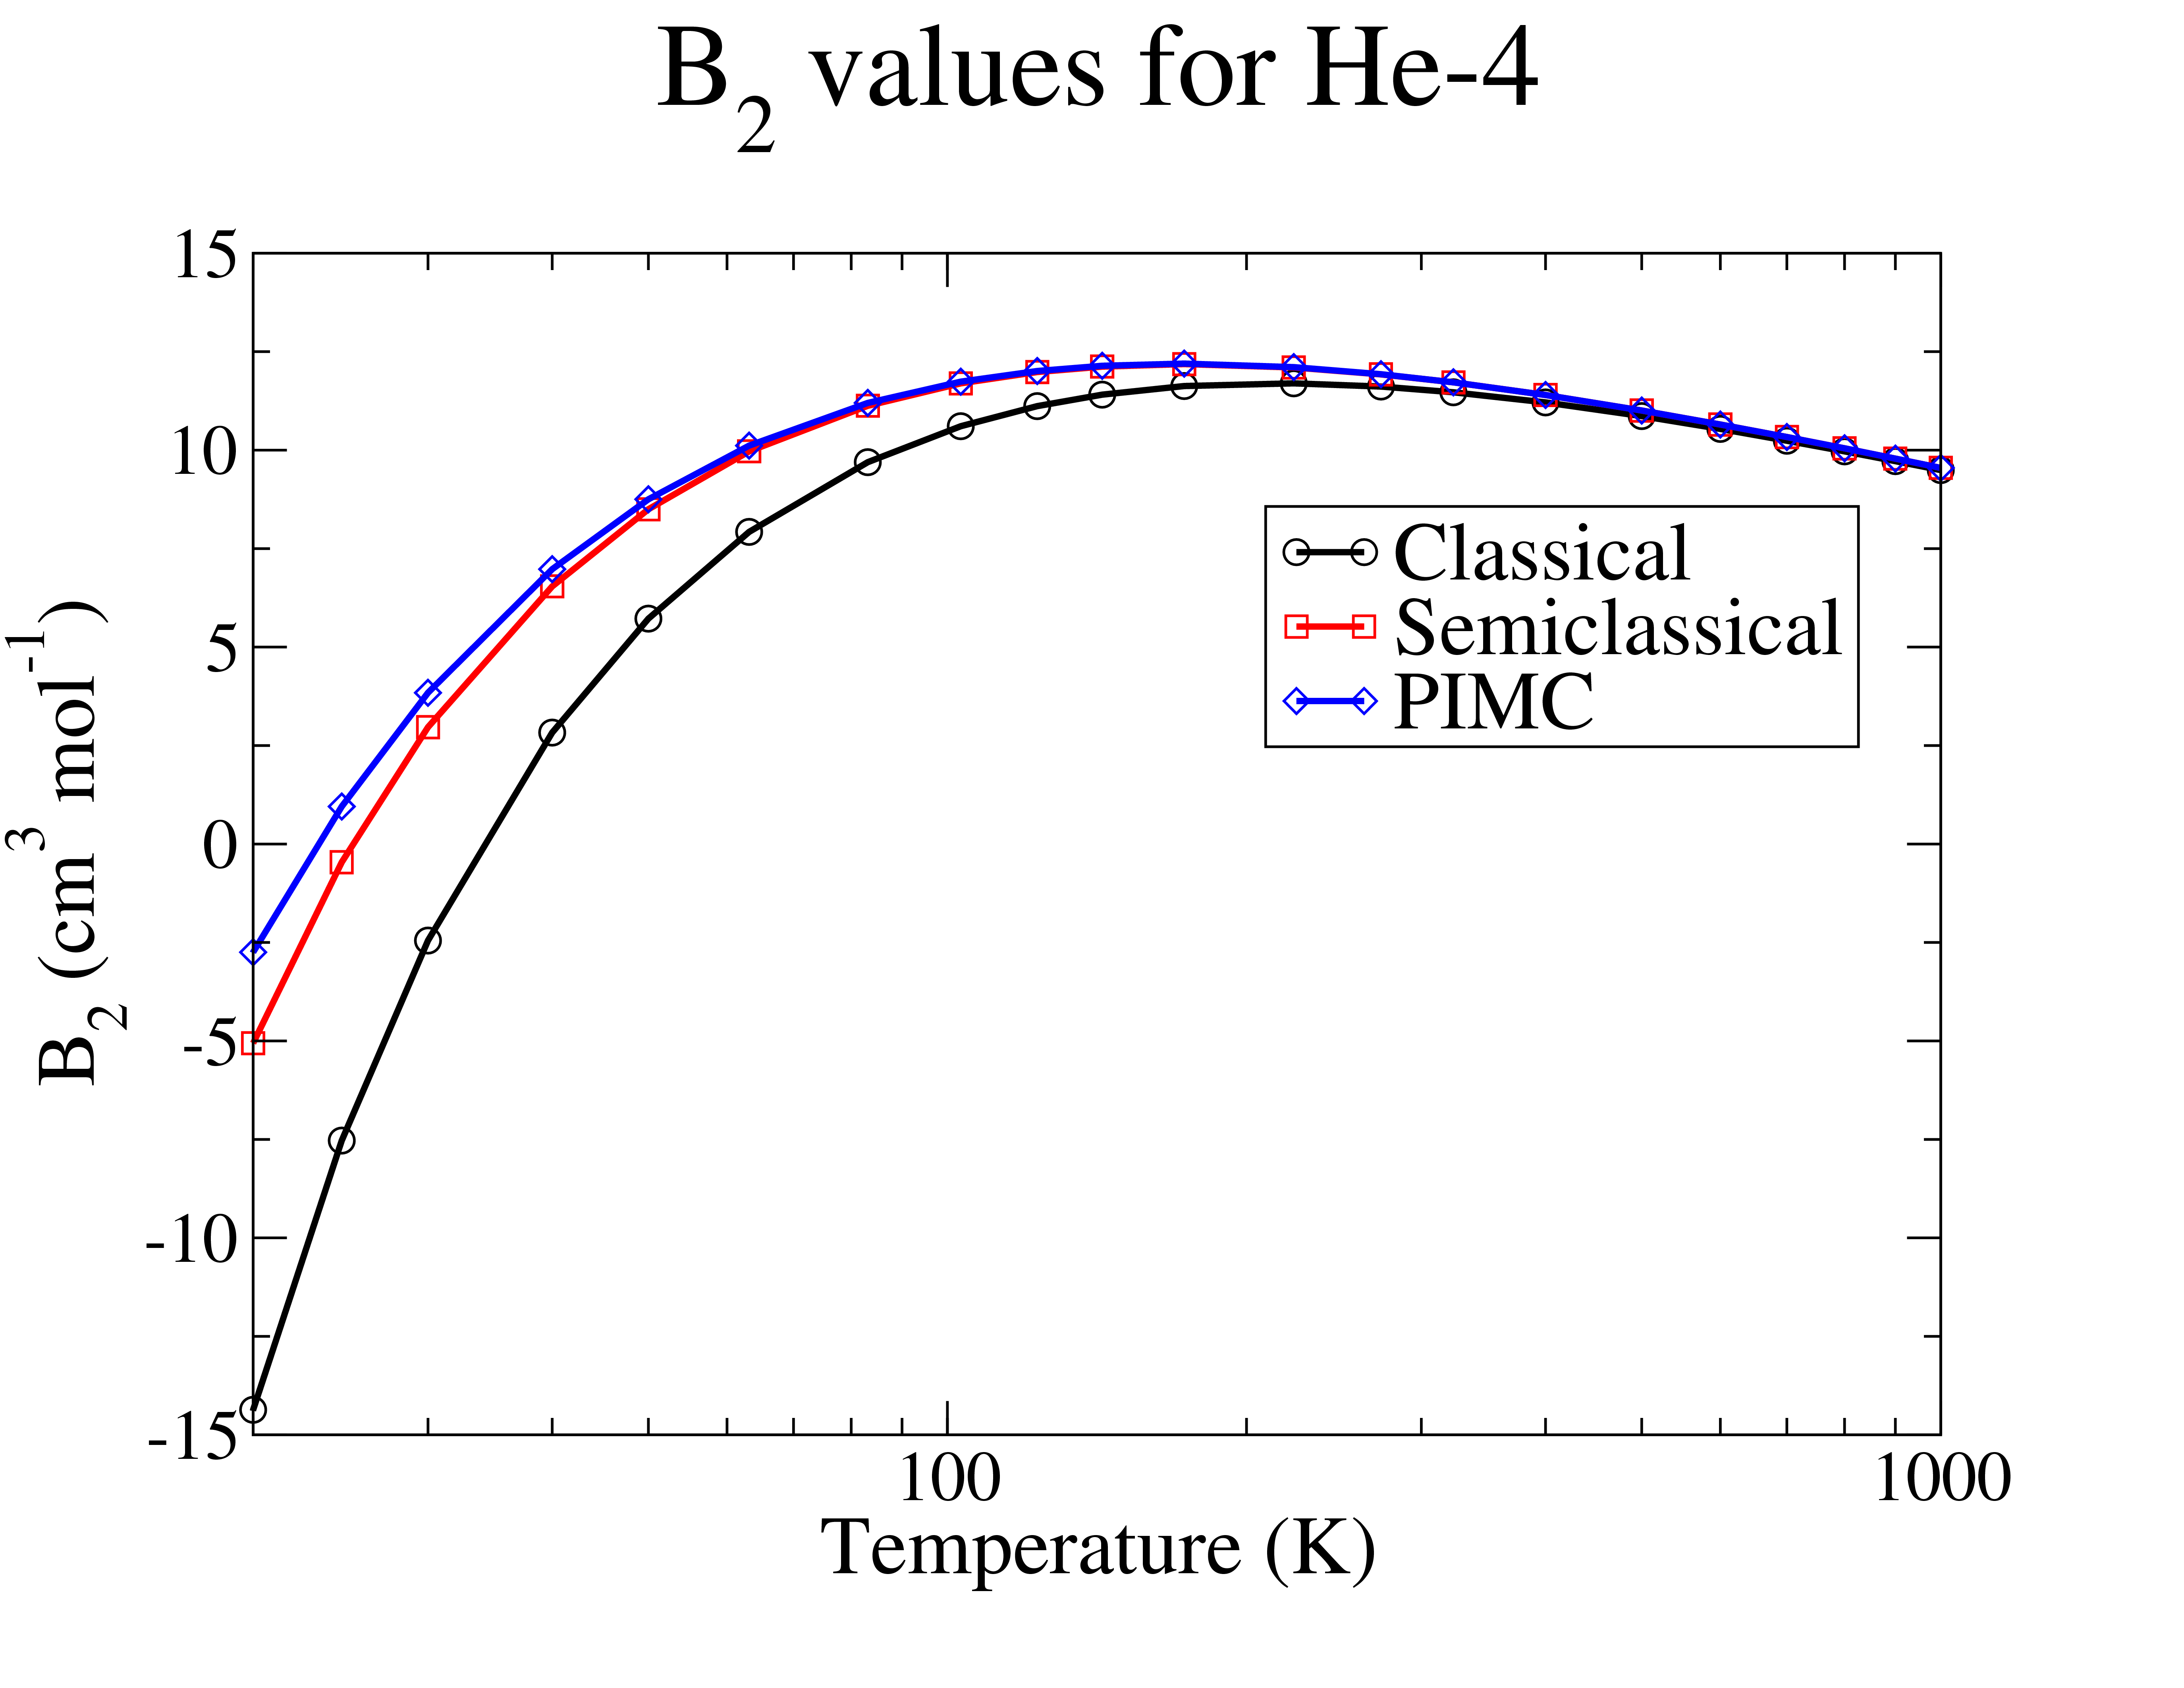
\includegraphics[scale=0.17,keepaspectratio]{B2-Kate.png}
            \end{figure}
        \end{frame}
	
    \section{Objectives}
        \begin{frame}
            \frametitle{Objective}
            \begin{block}{Diatomic molecules}
                Compute accurate virial coefficients using state-of-the-art \abinitio{} potentials and PIMC method.
            \end{block}
        \end{frame}
	\section{Methods}
	\subsection{Mayer Sampling Monte Carlo}
        \begin{frame}
            \frametitle{Mayer Sampling Monte Carlo}
            \begin{itemize}
            \justifying
                \item Second and third order virial coefficients are given by:
                \begin{equation*}
                    \begin{aligned}
                        B_2(T) &= -\frac{1}{2} \displaystyle\int d1 ~ f(0,1)\\
                        B_3(T) &= -\frac{1}{3} \displaystyle\int \int d1~d2~f(0,1)~f(0,2)~f(1,2)
                    \end{aligned}
                \end{equation*}
                \item MSMC\putCitation{Singh2004} is a free energy perturbation technique to evaluate the integrals in the above equations indirectly.
                \begin{equation*}
                    \label{eq:MSMCworking}
                    \begin{aligned}
                        \Gamma (T) &= \Gamma_o \frac{{<\gamma/\pi>}_\pi / {<\gamma_{os}/\pi>}_\pi}{{<\gamma_o/\pi>}_{\pi_o} / {<\gamma_{os}/\pi_o>}_{\pi_o}}\\
                        \gamma_{os} &= \frac{|\gamma_o||\gamma|}{\alpha |\gamma_o| + |\gamma|}
                    \end{aligned}
                \end{equation*}
            \end{itemize}
        \end{frame}
	\subsection{Path Integral Monte Carlo}
        \begin{frame}
            \frametitle{PIMC - thermal density matrix}
            \begin{itemize}
                \justifying
                \item The paritition function is an important property in statistical mechanics:
                \begin{equation*}
                    \begin{aligned}
                        P(x) &= \frac{1}{Z} \rho(x,x),\\
                        Z &= \int \rho(x,x) dx \equiv \text{trace} \{\rho\}.
                    \end{aligned}
                \end{equation*}
                where $\rho(x',x)$ is the statistical thermal density matrix at temperature T.
                \item Richard Feynman\putCitation{Feynman} was able to connect it with quantum mechanics:
                \begin{equation*}\label{eq:rho}
                    \rho (R , R' ; \beta) = < R | e^{- \beta \mc{H} } | R' >
                \end{equation*}
                where $R = \{\bm{r}_1, \bm{r}_2, \ldots \bm{r}_n\}$ and $\beta = 1/k_{\rm B}T$, with $k_{\rm B}$ Boltzmann's constant and $T$ the temperature.
            \end{itemize}
        \end{frame}
        \begin{frame}
            \frametitle{Important equations}
            \begin{itemize}
                \justifying
                \item A key property of the density matrix is that the product of two density matrices is also a density matrix. Hence the convlution\putCitation{Ceperley1995}:
                \begin{equation*}\label{eq:dmProduct}
                    \rho (R_1, R_3 ; \beta_1 + \beta_2) = \displaystyle\int dR_2 \rho (R_1, R_2 ; \beta_1) \rho (R_2, R_3 ; \beta_2)
                \end{equation*}
                \visible<2->{\item As $\frac{\beta}{P} \to 0$ or equivalently as $PT \to \infty$, the ``primitive approximation'' is given by\putCitation{Cui1997}:
                \begin{equation*}\label{eq:primitiveApprox}
                    e^{- \frac{\beta}{P} (\mc{T} + \mc{V})} \approx e^{- \frac{\beta}{P} \mc{T}} e^{- \frac{\beta}{P} \mc{V}}
                \end{equation*}
                    }
                \visible<3->{
                \item The Trotter formula proves that this approximation does converge to the right result in the $P \to \infty$ limit and is given by:
                \begin{equation*}\label{eq:trotter}
                    e^{- \beta (\mc{T} + \mc{V})} = \lim_{P \to \infty} \Big[ e^{- \frac{\beta}{P} \mc{T}} e^{- \frac{\beta}{P} \mc{V}} \Big]^P
                \end{equation*}
                    }
            \end{itemize}
        \end{frame}

        \begin{frame}
            \frametitle{Diatomic molecule - rigid rotor\putCitation{Patkowski2008}}
            \begin{itemize}
                \justifying
                \item Let $m$ and $I$ denote the mass of the atom and moment of inertia of the rigid rotor respectively with $\Lambda_m = h/\sqrt{2\pi m k_B T}$. Its Hamiltonian is given by:
                    \begin{equation*}
                    \label{eq:hDiatomic}
                        \hat{h}_2 = \displaystyle\frac{\hat{\mbf{p}}^2}{2m} + \frac{\hat{\mbf{J}}_1^2}{2I} + \frac{\hat{\mbf{J}}_2^2}{2I} + \hat{U}(r,\Omega_1,\Omega_2)
                    \end{equation*}
                    where $\hat{\mbf{p}}$ is the momentum operator conjugated to the COM separation, $\hat{\mbf{J}}_1$ and $\hat{\mbf{J}}_2$ are the angular momentum operators, $\hat{U}(r,\Omega_1,\Omega_2)$ is the intermolecular potential function in terms of the COM distance $r$ and the orientation vectors $\Omega_1$ and $\Omega_2$.

            \end{itemize}
        \end{frame}

        \begin{frame}
            \frametitle{Diatomic molecule - rigid rotor\putCitation{Patkowski2008}}
            \begin{itemize}
                \item Use $\mbf{x}^i, \mbf{\Omega}_1^i, \mbf{\Omega}_2^i$ to denote the configuration of the $i^\text{th}$ rigid rotors,
            \end{itemize}
            \begin{block}{Matrix elements}
                \begin{equation*}
                    \begin{aligned}
                        \mc{T}^{i,i+1}_{\text{tra}} = \left< \mbf{x}^i \left| \exp \left(-\displaystyle\frac{\beta \hat{\mbf{p}}^2}{2 m P} \right) \right| \mbf{x}^{i+1} \right> &= \alert<2>{\displaystyle\frac{P^{3/2}}{\Lambda_m^3} \exp \left(-\displaystyle\frac{\pi P (\mbf{x}^i - \mbf{x}^{i+1})^2}{\Lambda_m^2}\right)}\\
                        \mc{T}^{i,i+1}_{\text{rot}} = \left< \Omega^i \left| \exp \left(-\displaystyle\frac{\beta \hat{\mbf{J}}^2}{2IP} \right) \right| \Omega^{i+1} \right> &= \alert<3>{\displaystyle\sum_{j=0}^\infty \frac{2j+1}{4 \pi} \mc{P}_j (cos (\theta_{i,i+1}))}\\
                        &\qquad \alert<3>{\times \exp \left[-\beta j(j+1) \Upsilon/ P \right]}
                    \end{aligned}
                \end{equation*}
                where $j$ is the angular quantum number, $\theta_{i,i+1}$ is the angle between bead orientation vectors $\Omega_i, \Omega_{i+1}$, $\mc{P}_j$ is the Legendre polynomial of order $j$ and $\Upsilon = \hbar^2/(2I)$.
            \end{block}
        \end{frame}

        \begin{frame}
            \frametitle{Diatomic molecule - rigid rotor\putCitation{Patkowski2008}}
            \begin{itemize}
                \justifying
                \item Defining $\mbf{r} \equiv \mbf{x}^{(1)}, \mbf{\Delta}^{(i)} \equiv \mbf{x}^{(i+1)} - \mbf{x}^{(i)}$,
                \begin{equation*}
                    \exp [-\beta \bar{U} (|\mbf{r}|) = \left< \exp \left[ -\frac{\beta}{P} \sum_{i=1}^P U (|\mbf{x}^i|,\Omega_1^i,\Omega_2^i) \right] \right>_{F,\varrho}
                \end{equation*}
                \item Probability distributions:
                \begin{align*}
                    \varrho(\mbf{\Omega}) &= \frac{1}{q_\text{rot}} \displaystyle\prod_{i=1}^P \mc{T}_\text{rot}^{i,i+1}, \qquad F(\mbf{\Delta}) = \Lambda_m^3 \displaystyle\prod_{i=1}^P \mc{T}_\text{tra}^{i,i+1}\\
                    q_{rot} &= \displaystyle\sum_{j'} (2j' + 1) \exp \left[-\beta \Upsilon j' (j'+1) \right]
                \end{align*}
            \end{itemize}
            \begin{block}{Fully quantum second virial coefficient}
                \begin{equation*}
                    \alert{B_2 (T) = -2 \pi \displaystyle\int dr~ r^2 (e^{-\beta \bar{U} (r)} - 1)}
                \end{equation*}
            \end{block}
        \end{frame}
        \begin{frame}
            \frametitle{Objectives}
            \begin{block}{Diatomic molecules}
                Compute accurate virial coefficients using state-of-the-art \abinitio{} potentials, MSMC and PIMC methods.
            \end{block}
            \begin{alertblock}{Challenges}
                Lack of efficient an sampling algorithm for orientations.
            \end{alertblock}
        \end{frame}

        \begin{frame}
            \frametitle{Objectives}
            \begin{block}{Diatomic molecules}
                Compute accurate virial coefficients using state-of-the-art \abinitio{} potentials, MSMC and PIMC methods for the rigid case.
            \end{block}
                \begin{alertblock}{Challenges}
                    inability to include vibrational degrees of freedom under the assumption of rigid rotors.
                \end{alertblock}
        \end{frame}
        \subsection{Novel algorithms}
        \begin{frame}
            \frametitle{Orientation sampling}
            \begin{itemize}
                \item Idea proposed by Garberoglio et al. \cite{Garberoglio2014}: two independent atoms (vs. one rigid rotor previously)
                \item Calculate the probability distribution as:

            \end{itemize}
        \end{frame}

	\section{Results}
	\section{Summary}
	\section*{Ackowledgements}

	\begin{frame}
	\frametitle{PIMC - diatomic molecule}
	\begin{itemize}
	\justifying
	\item PIMC - provides a route to incorporate nuclear quantum effects
	\item Kinetic energy effects of the molecule lead to harmonic spring-like interactions between adjacent ``beads"
	\begin{figure}
	\centering
	\def\svgscale{0.3}
	\input{monatomicPIMC.pdf_tex}
	\end{figure}
	\item Interaction energy is computed as: $U_{int} = \displaystyle\sum\limits_{i=1}^P \frac{U_i}{P}$
	\begin{figure}
	\centering
	\def\svgscale{0.3}
	\input{interactionEnergyMonatomic.pdf_tex}
	\end{figure}
	\item To form a closed ring of springs, the position of each bead needs to be chosen based on a Gaussian distribution. Hence, implementing PIMC is trivial for the monatomic case
	\end{itemize}
	\end{frame}
	
	\begin{frame}
	\frametitle{PIMC results for Helium-4\putCitation{Shaul2012}}
	\begin{figure}
	\centering
	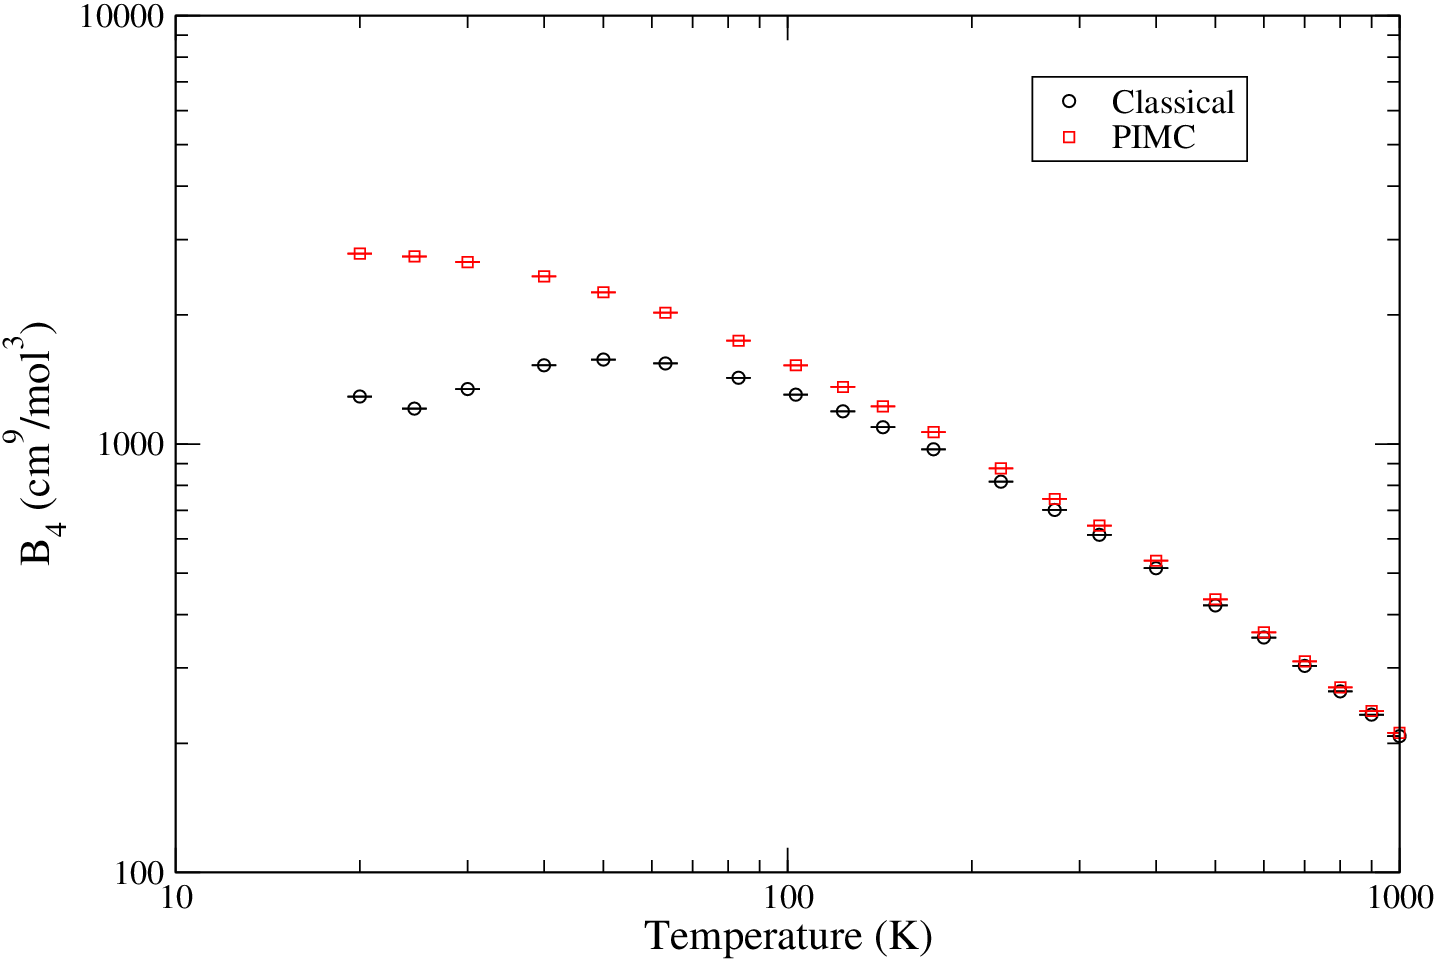
\includegraphics[scale=0.2,keepaspectratio]{B4-Kate.png}
	\end{figure}
	\end{frame}

	\begin{frame}
	\frametitle{PIMC - rigid diatomic molecule}
	\begin{itemize}
	\item Probability distribution for choosing an orientation is not Gaussian
	\item Probability of choosing adjacent orientation is exact and analytic but we can't form a ring if we choose from that distribution
	\begin{figure}
	\centering
	\def\svgscale{0.2}
	\input{orientationRD.pdf_tex}
	\end{figure}
	\item Entire difficulty lies in coming up with a probability distribution for non-adjacent monomer orientations which results in closed ring configurations
	\begin{figure}
	\centering
	\def\svgscale{0.3}
	\input{diatomicPIMC.pdf_tex}
	\end{figure}
	\end{itemize}
	\end{frame}
	
	\begin{frame}
	%slide 8
	\frametitle{A new orientational sampling algorithm}
	\begin{itemize}%[<+->]
	\item What if we don't model using the quantum rigid rotor approximation?
	\item The only factor that affects the probability of any configuration is the \alert{harmonic spring-like interaction} between adjacent beads
	\item $U_h = \displaystyle\sum\limits_{\# rings} \displaystyle\sum\limits_i k_h |\textbf{x}_i - \textbf{x}_{i-1}|^2 ,\text{with} \: k_h = \frac{\pi P}{\Lambda^2}$ where $\Lambda = \frac{h}{\sqrt{2 \pi m k_B T}}$ \: and $\textbf{x}_i$ denotes position of the bead $i$
	\item The actual probability of any configuration is given by $P_{act} = exp(-U_h) $
	\end{itemize}
	\end{frame}

	\begin{frame}
	\frametitle{Growing the ring}
	\begin{itemize}%[<+->]
	\item Tight coupling between adjacent beads makes it difficult to sample orientations that are different, thus lowering the sampling efficiency
	\item We always \alert{grow the complete ring each time} and  we do so \alert{non-sequentially}
	\end{itemize}
	\end{frame}

	\begin{frame}
	\frametitle{Non-sequential algorithm}
	%slide 9
	\begin{itemize}%[<+->]
	\begin{columns}[c]
	\column{6cm}
	\item Image 0 and image P are one and the same. The choice of orientation of image 0 is arbitrary
	\item Each image(child) has a set of two(parent) orientations which affect where it is placed
	\item For each pass, we need a probability distribution of the child image that depends on the orientations of both the parent images

	\column{3.4cm}
	\vspace{0cm}
	\begin{overlayarea}{3.5cm}{3.5cm}
	\begin{figure}[H]
	\only<1>{
	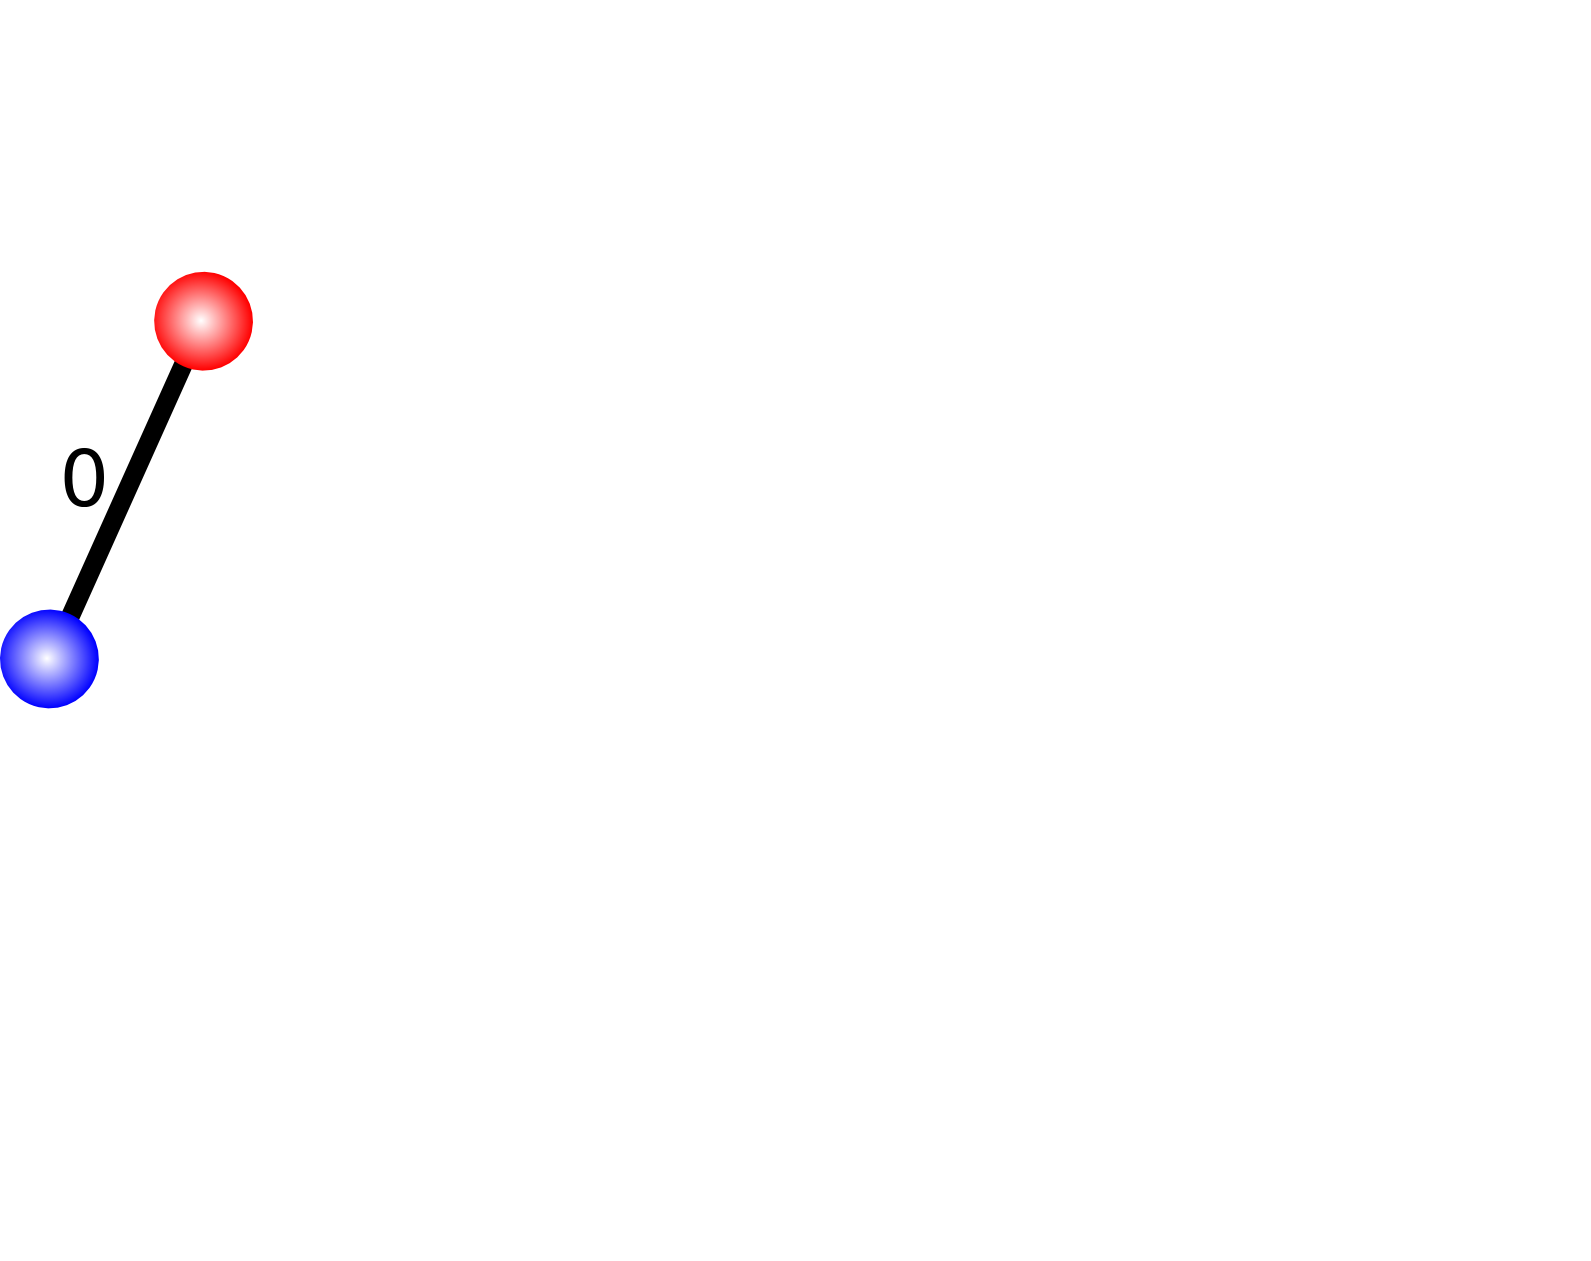
\includegraphics[width=3.5cm,height=3.5cm,keepaspectratio]{ns0.png}
	\caption{Example for P = 8}
	}
	\only<2>{
	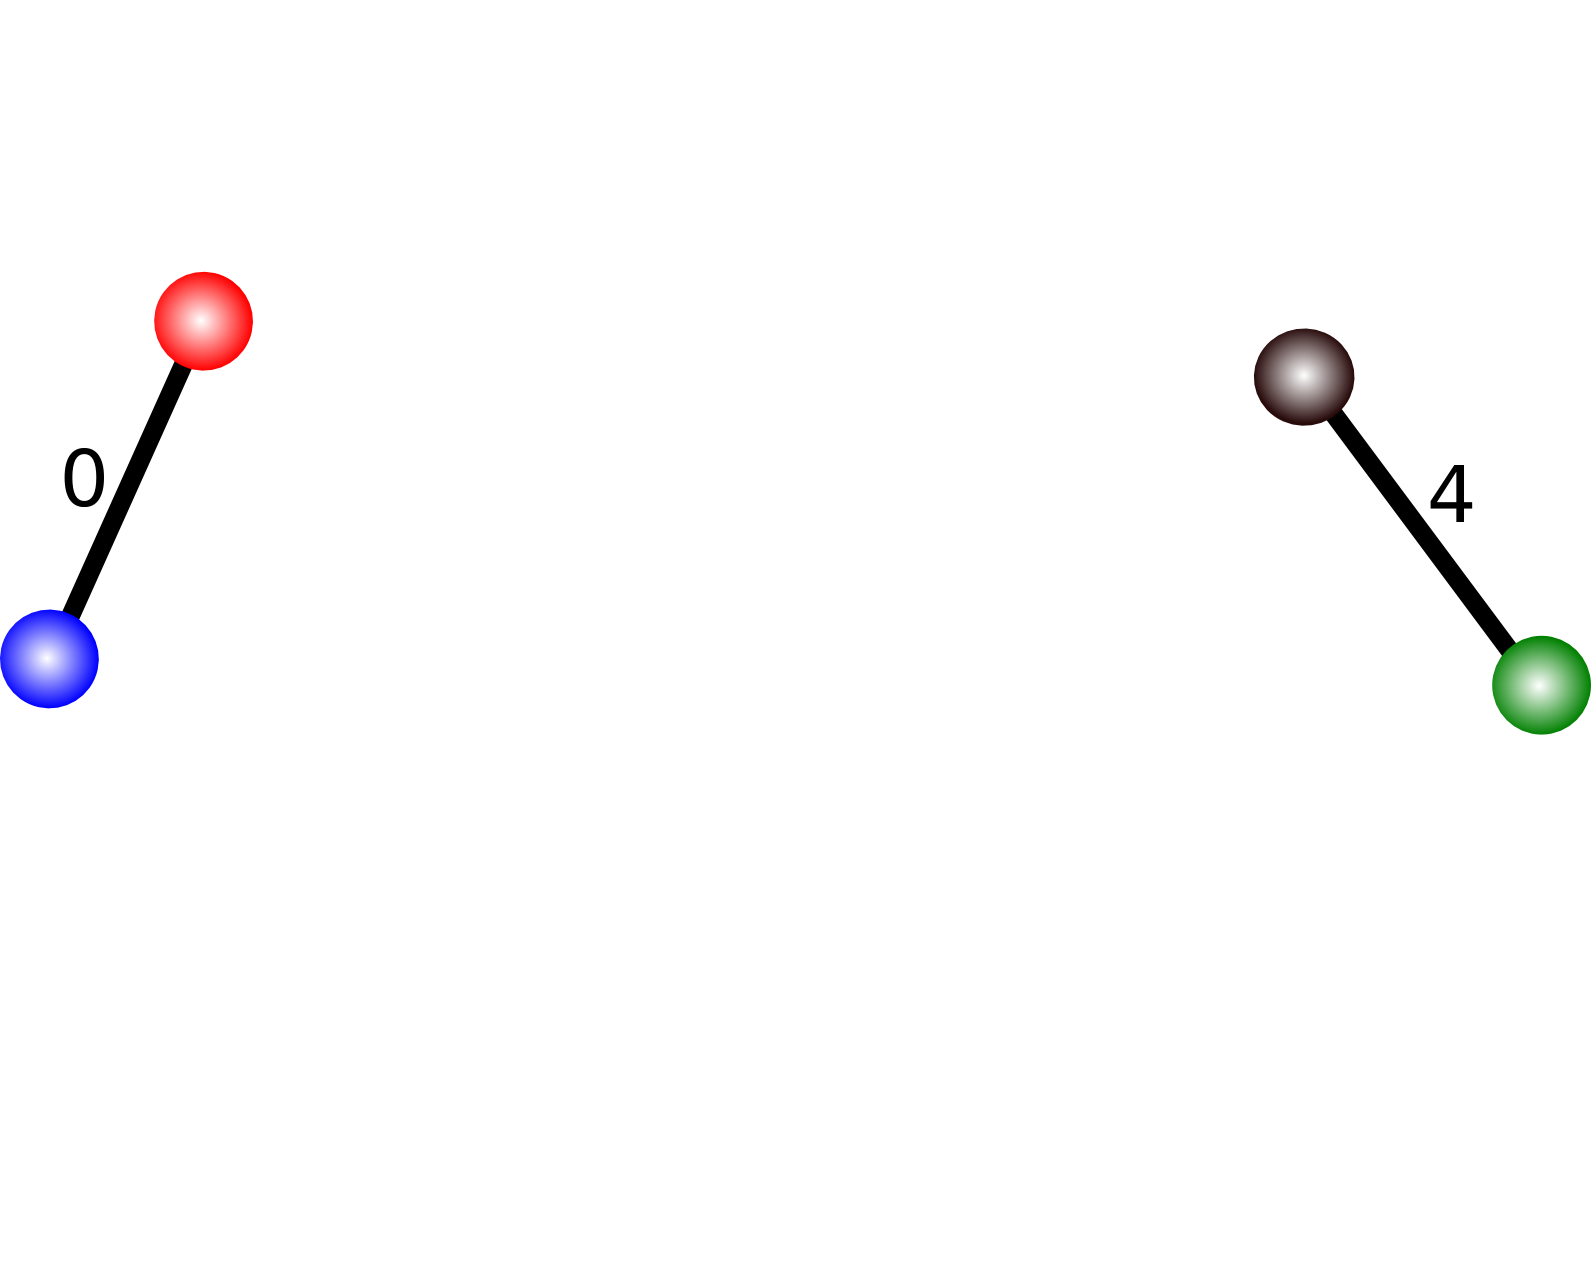
\includegraphics[width=3.5cm,height=3.5cm,keepaspectratio]{ns04.png}
	\caption{Example for P = 8}
	}
	\only<3>{
	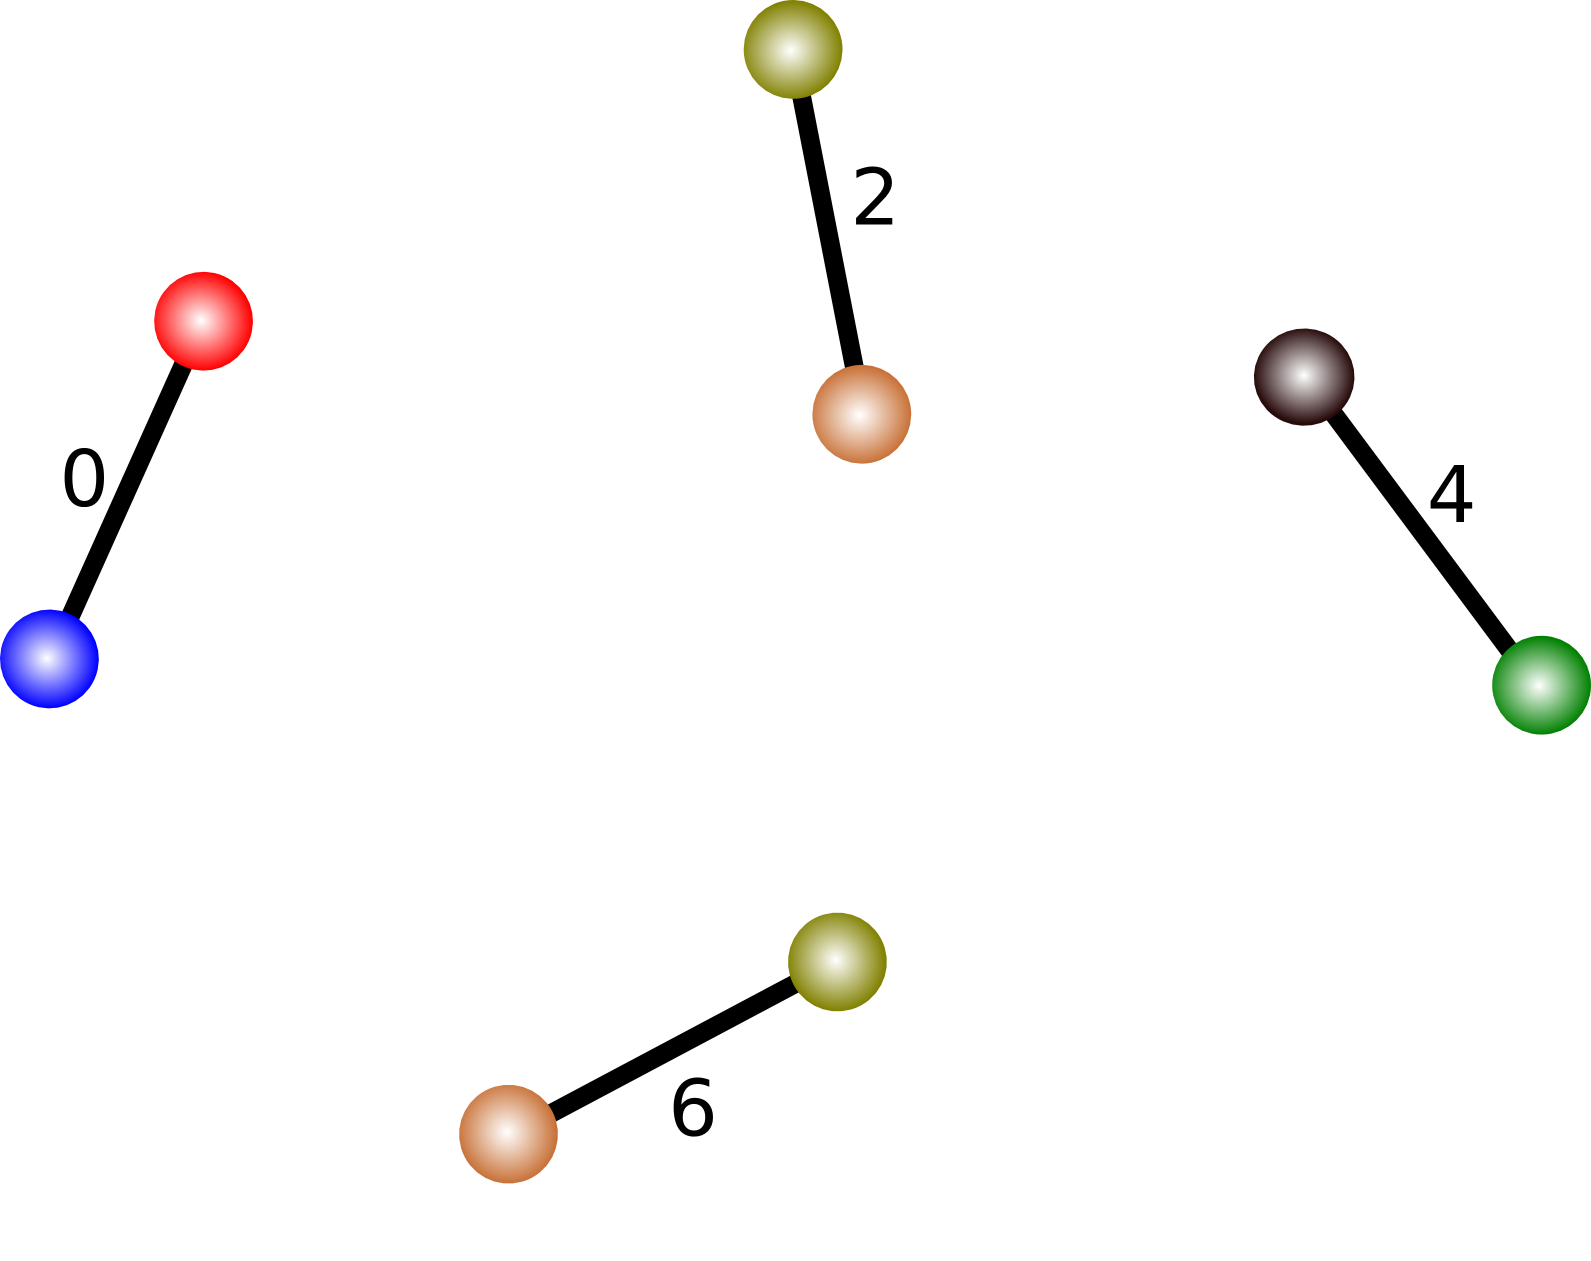
\includegraphics[width=3.5cm,height=3.5cm,keepaspectratio]{ns0426.png}
	\caption{Example for P = 8}
	}
	\only<4>{
	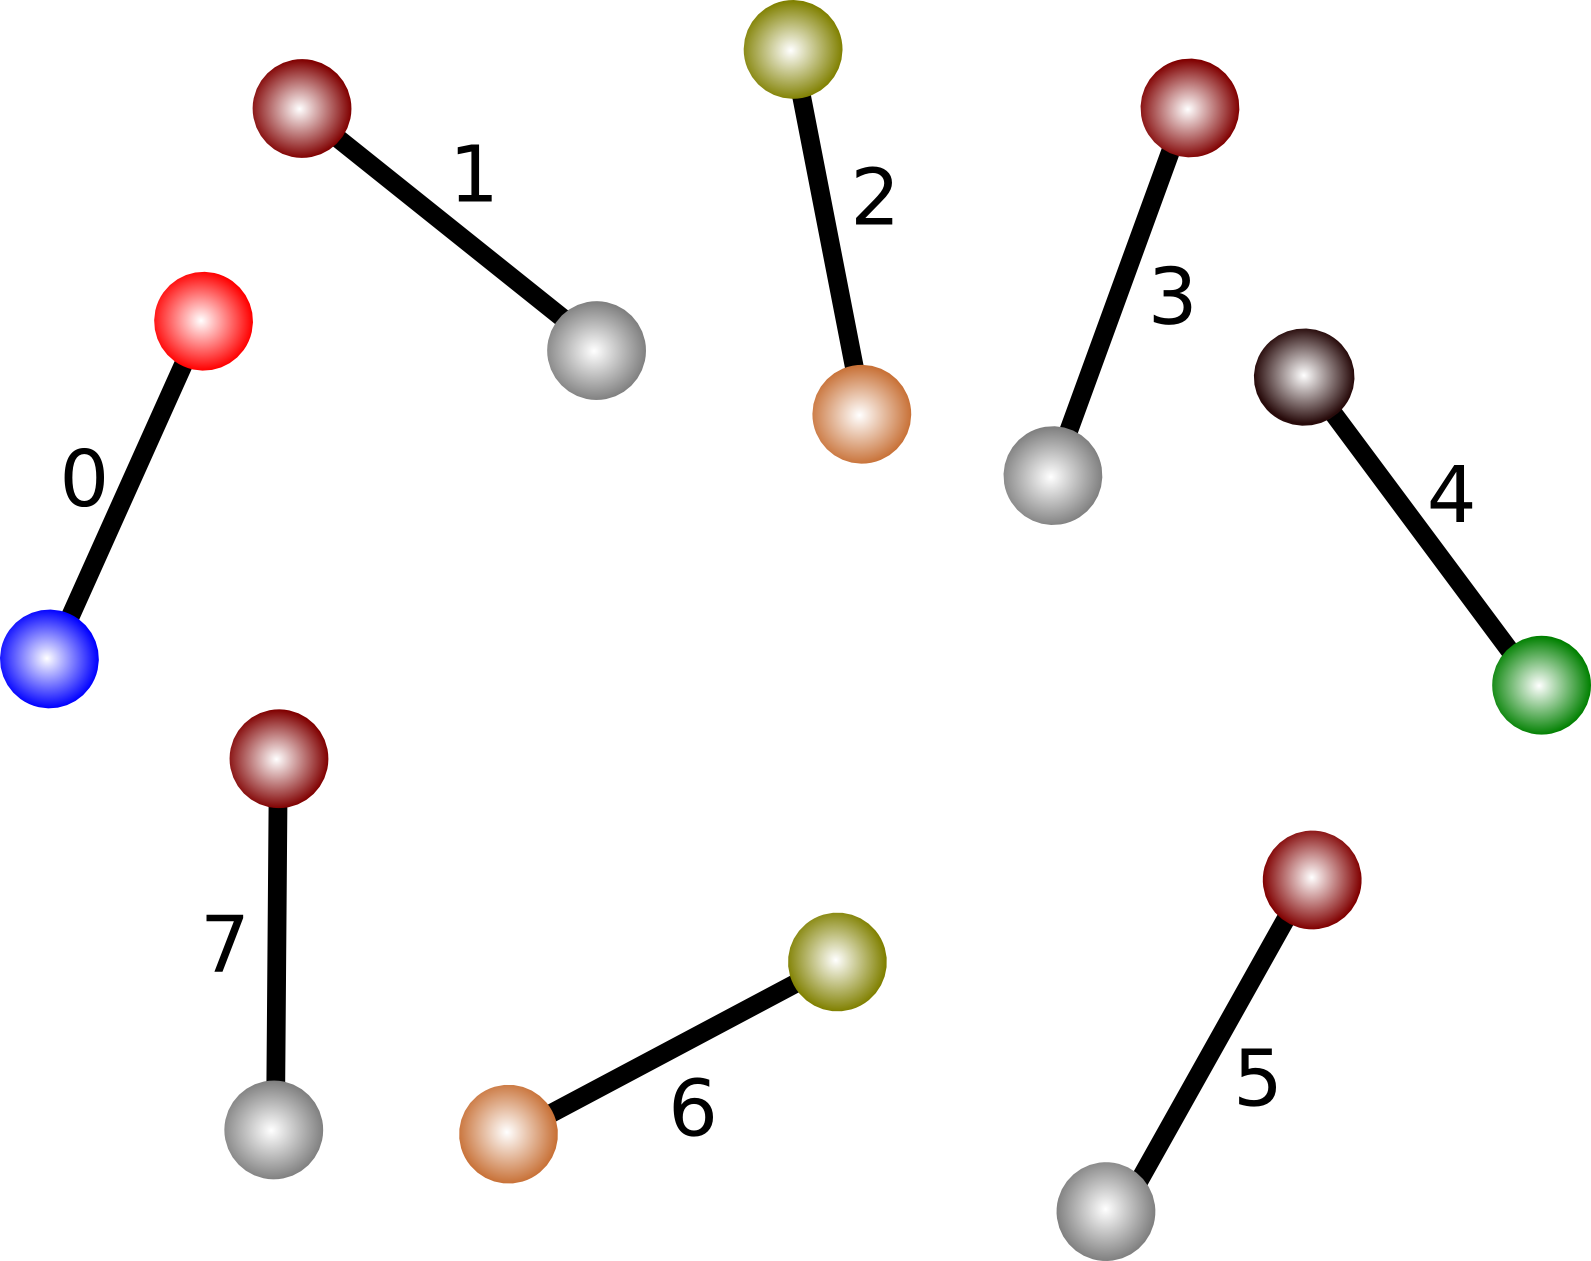
\includegraphics[width=3.5cm,height=3.5cm,keepaspectratio]{nsall.png}
	\caption{Example for P = 8}
	}
	\end{figure}
	\end{overlayarea}
	\end{columns}
	\end{itemize}
	\end{frame}

	\begin{frame}
	%slide 10
	\frametitle{Adjacent image probability $P_{01}$}
	\begin{itemize}%[<+->]
	\begin{columns}[t]
	\column{6cm}
	\item Consider a sphere with diameter $=$ bond length of the molecule i.e. $r = b/2$
	\item Let image `0' be oriented along the z-axis and image `1', at angle \:$\phi_1$\: away from it
	\item Distance `x' between beads of adjacent images is given by $x^2 = 2 r^2 ( 1 - cos \phi_1)$
	\column{3.4cm}
	\begin{figure}
	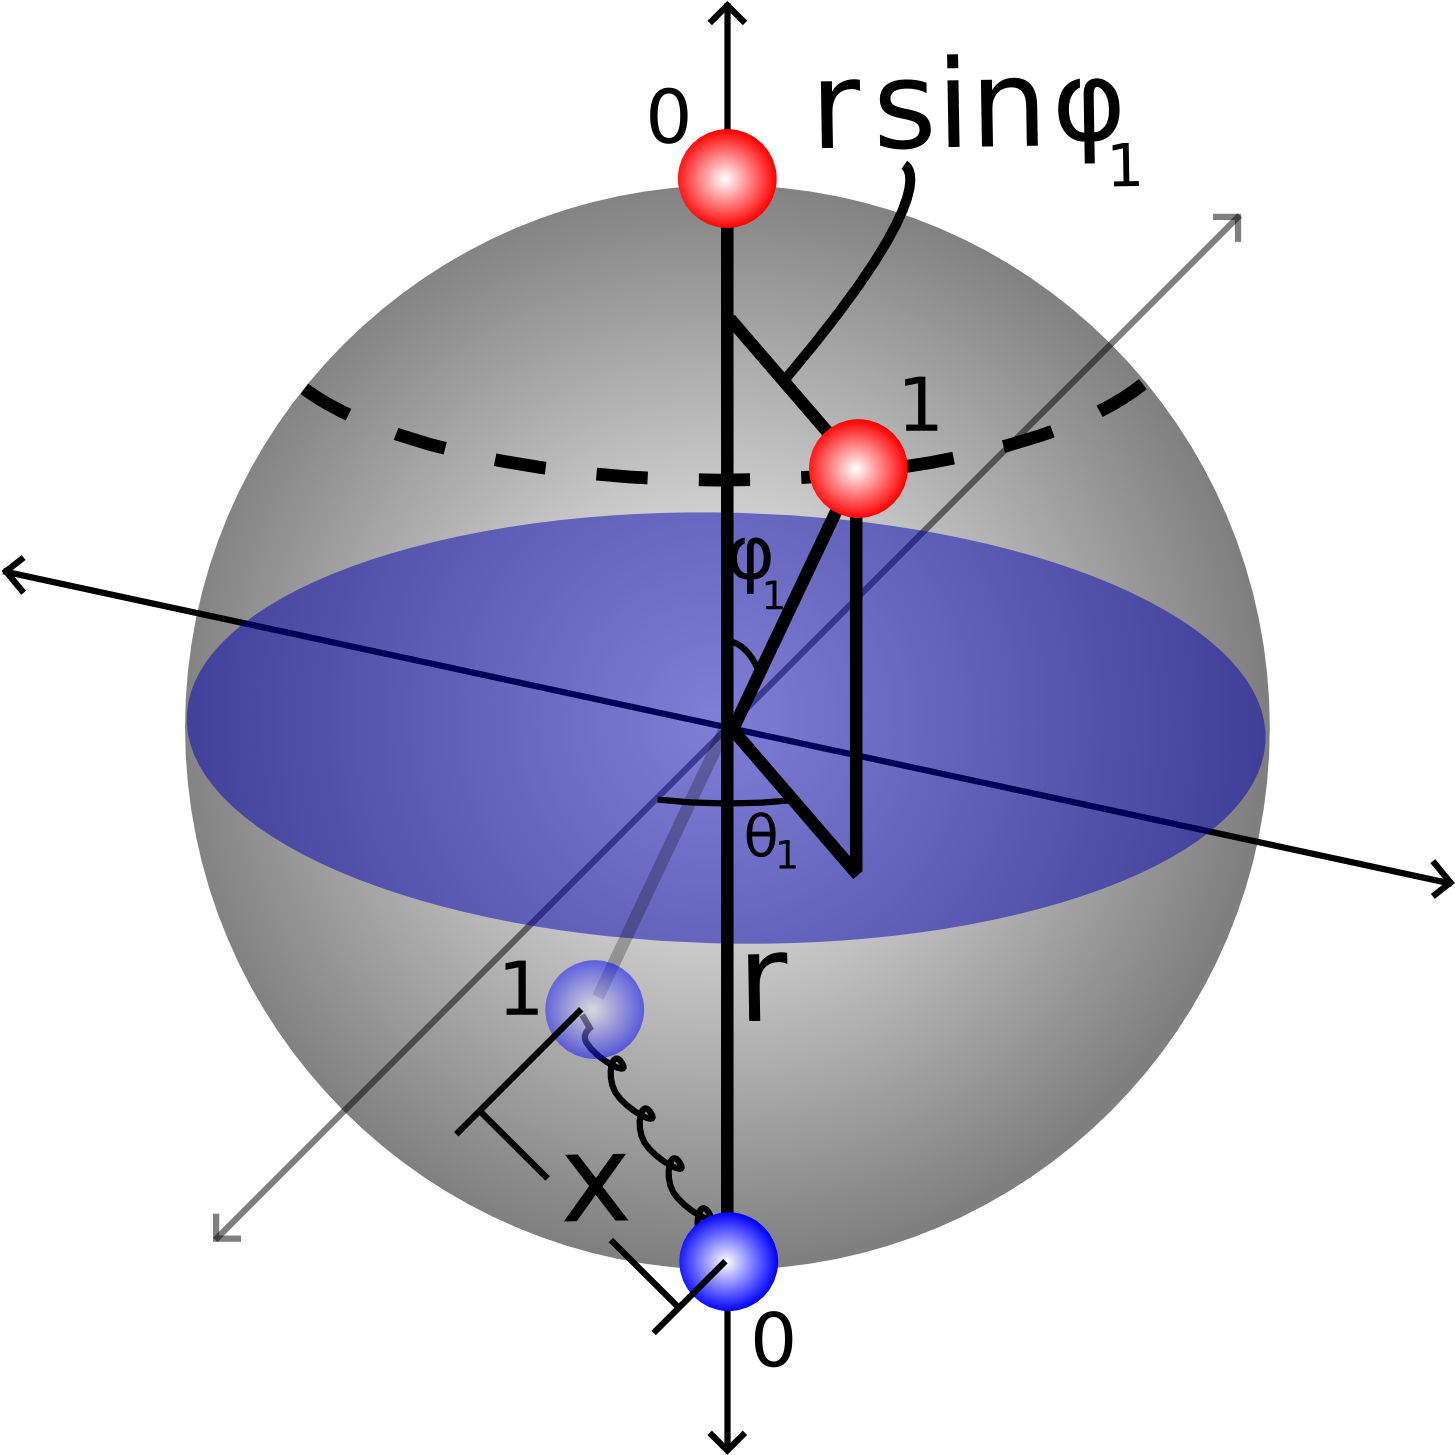
\includegraphics[width=\textwidth,keepaspectratio]{degeneracyNew.png}
	\caption{P = 2 case}
	\end{figure}
	\end{columns}
	\item The harmonic interaction energy is given by, $U_h = 4 k_h r^2 (1 - cos \phi_1)$
	\item $P_{01}$ is given by:
	\begin{align}
	P_{01} (\phi_1) = exp [-4k_h r^2 (1 - cos \phi_1)]
	\end{align}
	\end{itemize}
	\end{frame}

	\begin{frame}
	%slide 11
	\frametitle{Comparison between algorithms\putCitation{Patkowski2008}}
	Normalize these the two functions $P_{01}, \rho$ :
	\begin{align*}
	P_{01} (\phi_1) = &exp [ -4 k_h r^2 (1 - cos \phi_1) ] \\
	\rho(\phi_1) = &\frac{1}{q_{rot}} \displaystyle\sum\limits_{j=0}^{100} \frac{2j+1}{4 \pi} P_j (cos \phi_1) \times exp[- \beta j (j+1)\Upsilon /P]
	\end{align*}
	\begin{center}
	\begin{figure}
	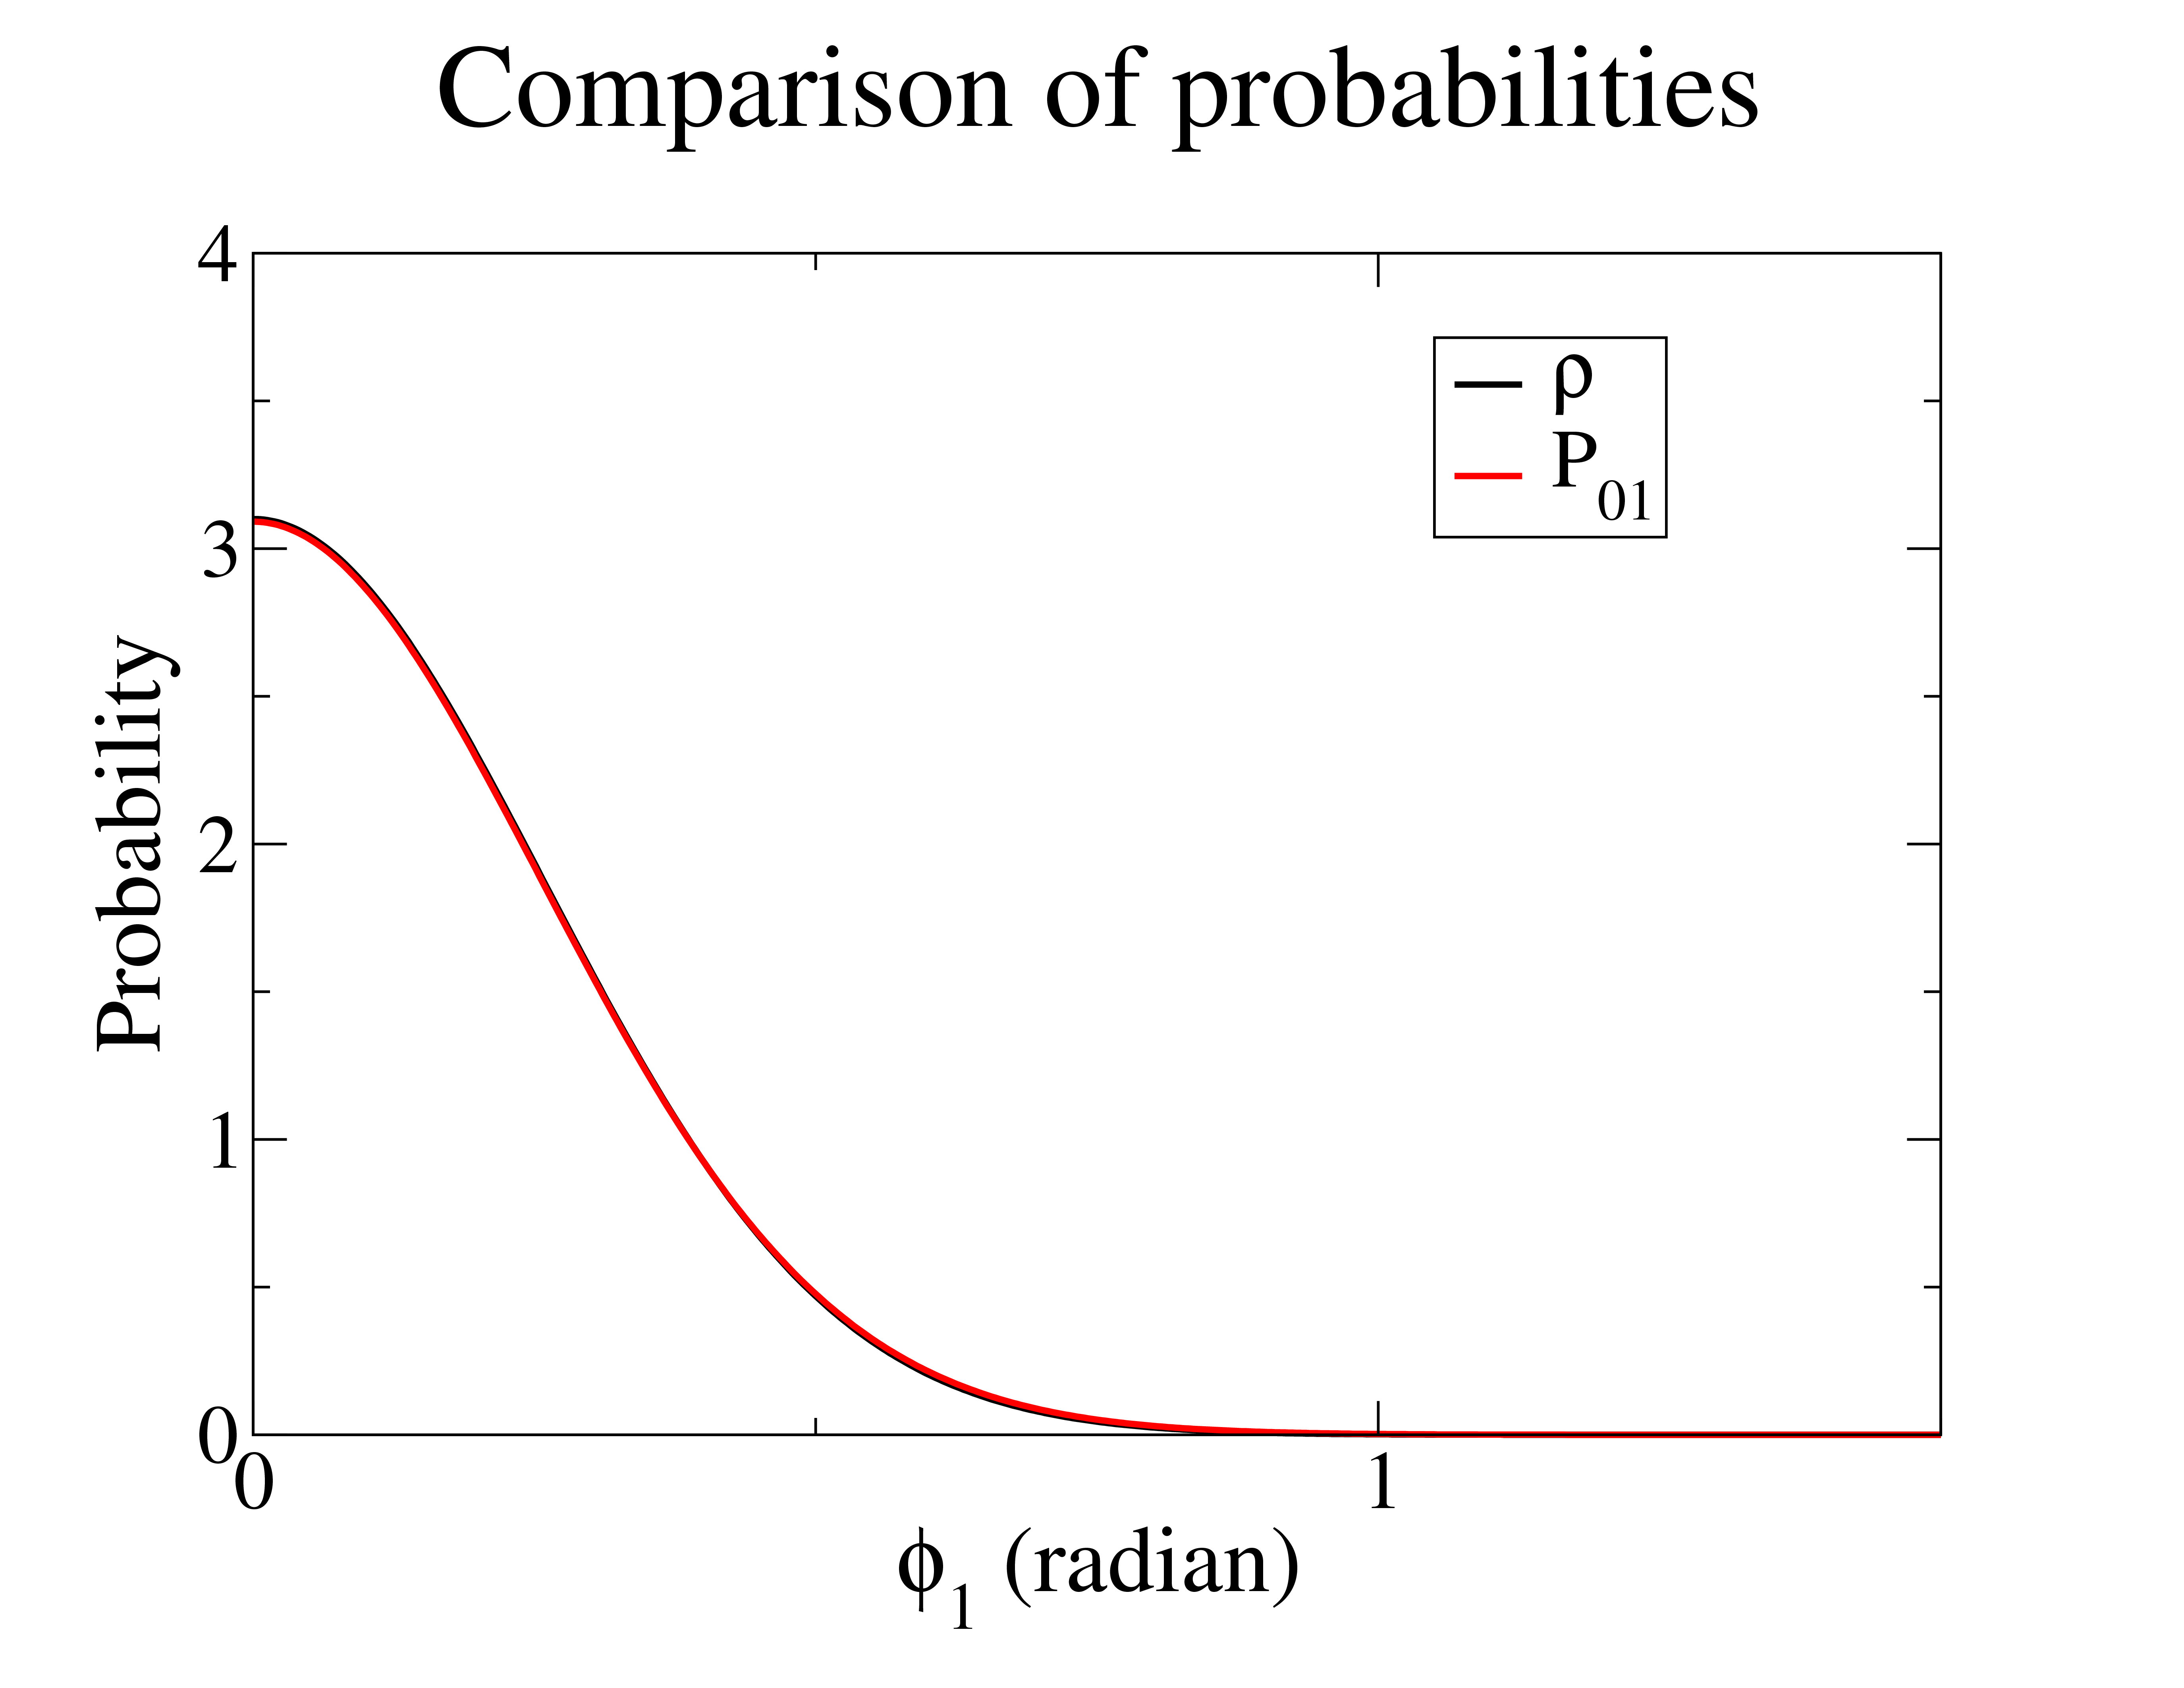
\includegraphics[width=5.5cm,keepaspectratio]{probabilityComparison.png}
	\end{figure}
	\end{center}
	\end{frame}

	\begin{frame}
	%slide 12
	\frametitle{Parent $\to$ child}
	\begin{itemize}%[<+->]
	\item Given two parent images $I_1,I_2$, the harmonically most favorable orientation for the child image is the average of the their orientations
	\item Let $c_n$ denote the average orientation of the two parents for image n and $P_{c_n,I_1 I_2}$ denote the probability distribution centered around $c_n$
	\item For the case of $n = 1, P_{c_1,02}$ can be computed analytically
	\begin{center}
	\begin{figure}
	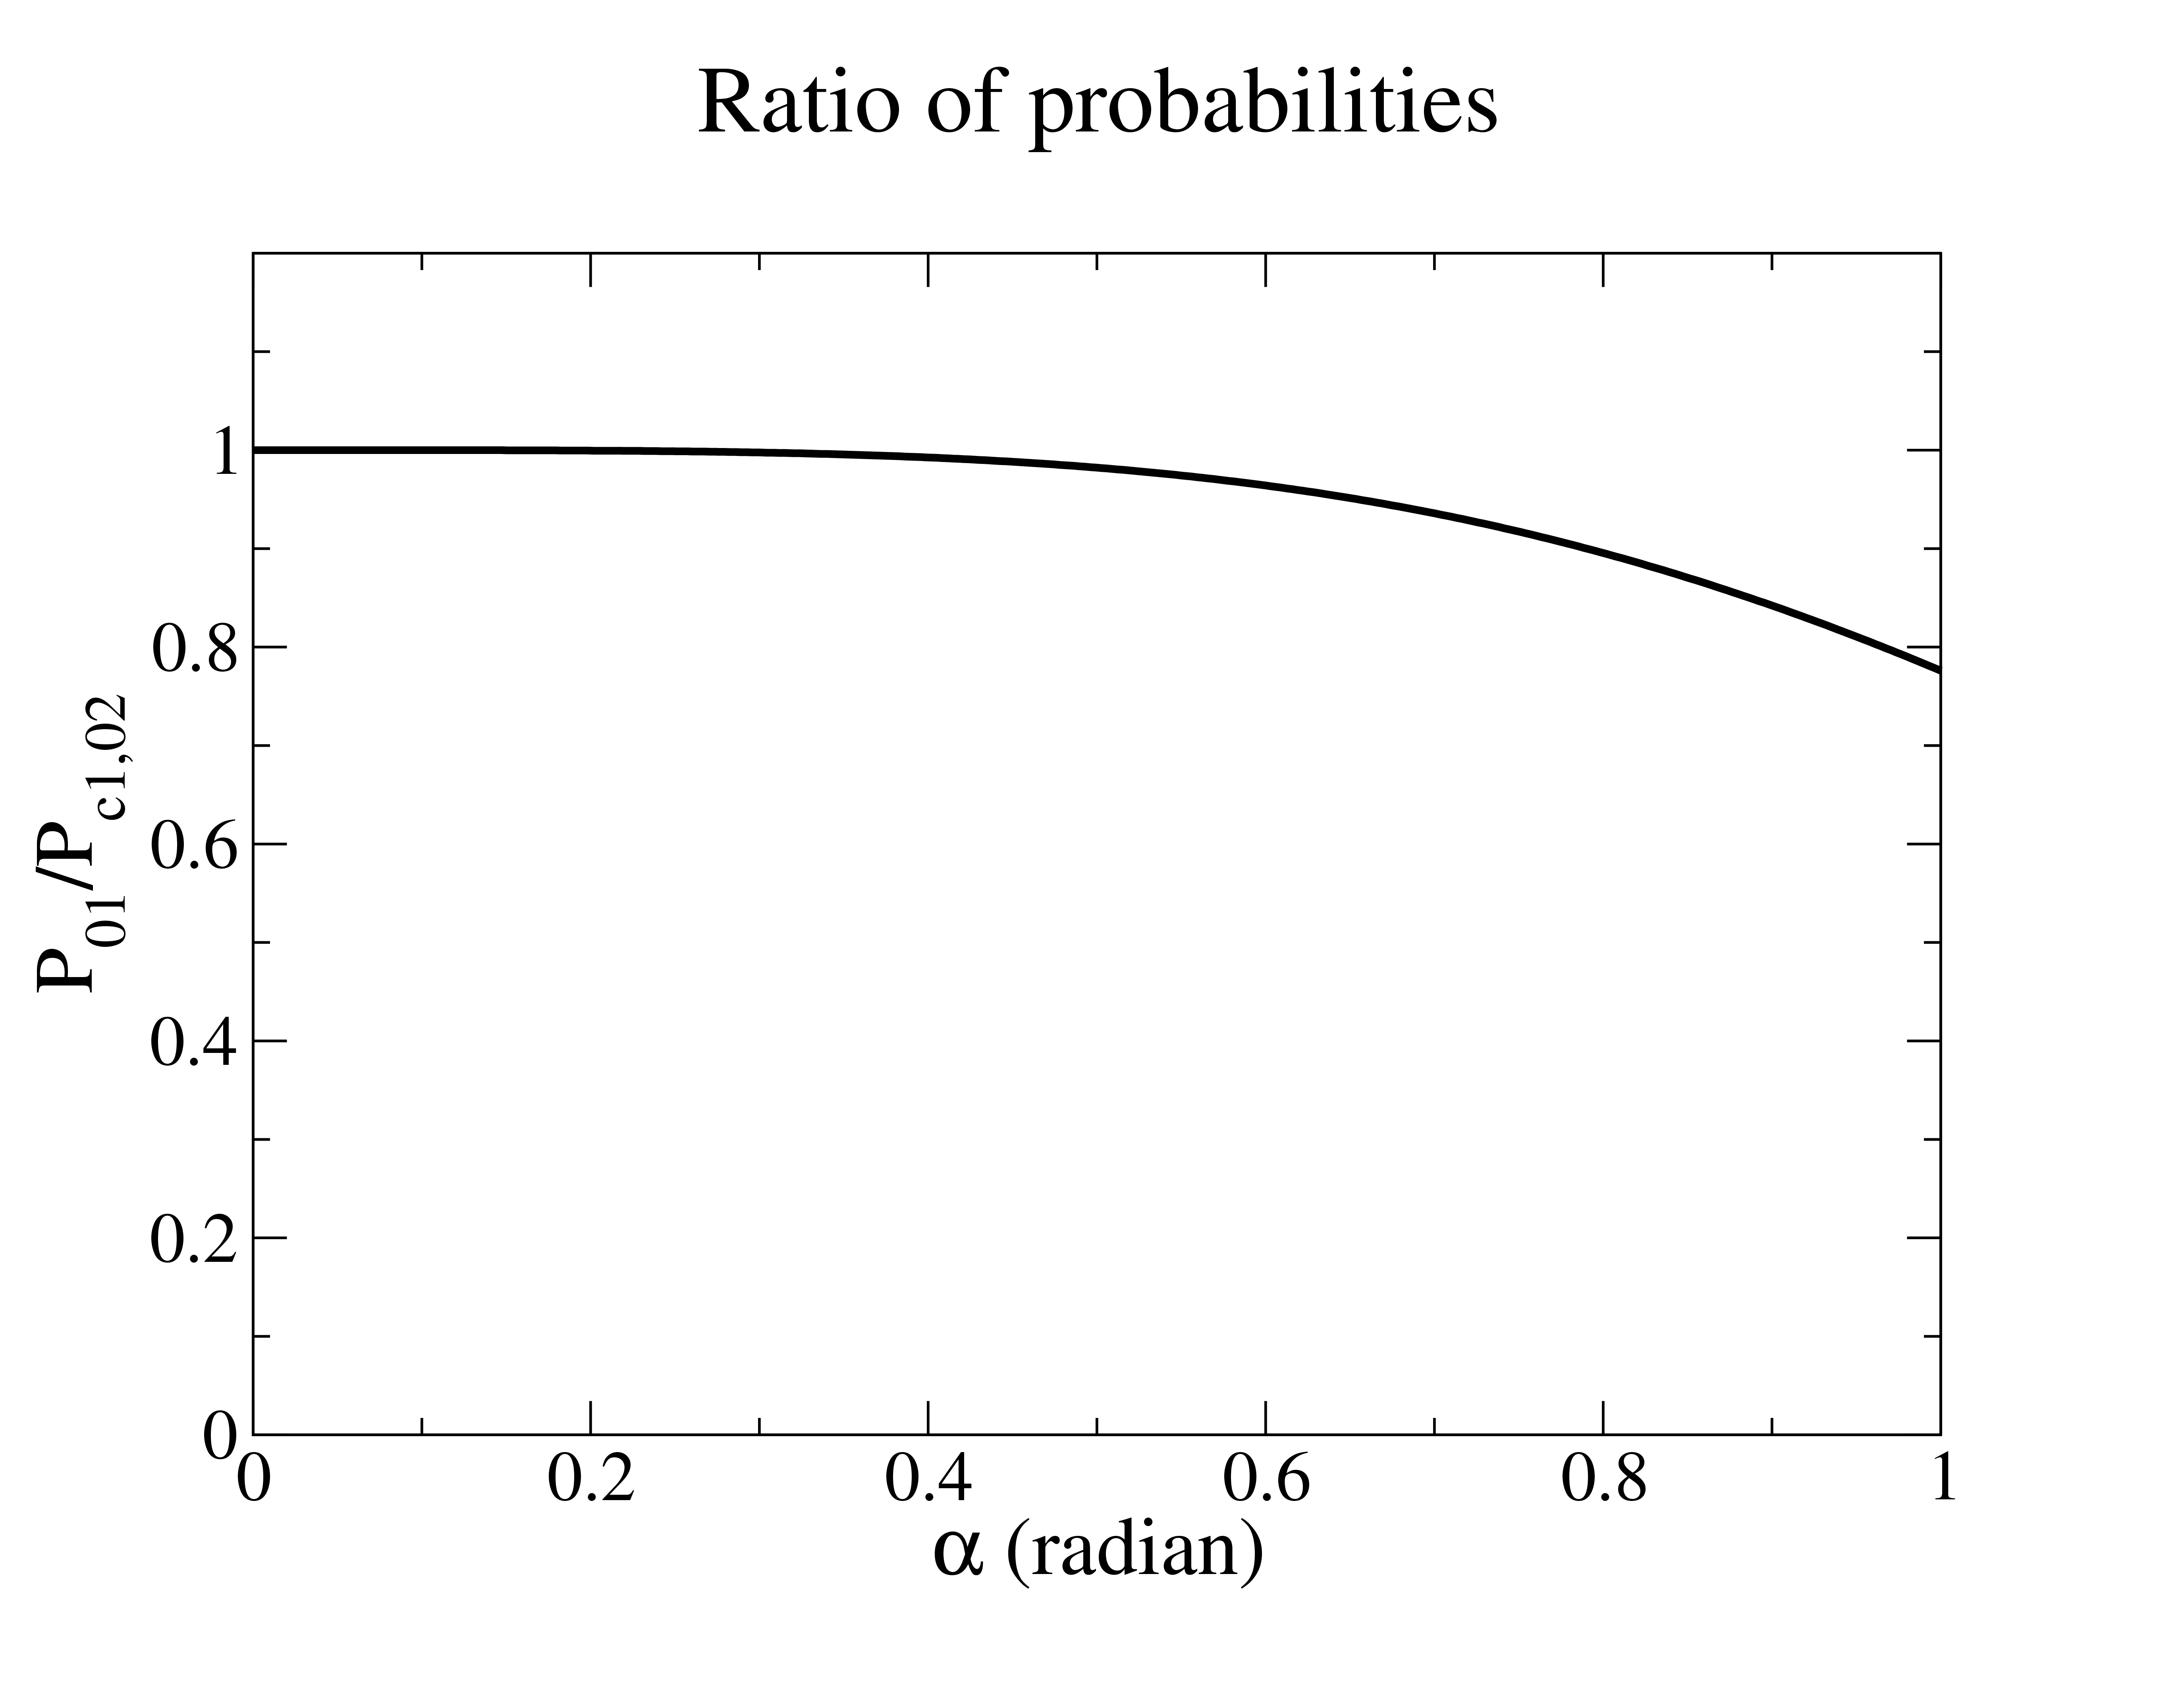
\includegraphics[width=6cm,keepaspectratio]{yratio.png}
	\end{figure}
	\end{center}
	\end{itemize}
	\end{frame}

	\begin{frame}
	%slide 13
	\frametitle{Parent $\to$ child}
	\begin{itemize}%[<+->]
	\item We performed MC simulations and collected histograms of angles $\phi_2 , \phi_4, \phi_8 \ldots$ and observed that:
	\begin{align*}
	&P_{c_n,I_1 I_2} (\phi_n) \approx P_{01} (k_n^{eff},\phi_n) \\
	&k_n^{eff} \propto k_h cos(\psi_n/2)
	\end{align*}
	where $\psi_n$ is the angle between the orientations of $I_1 , I_2$
	\item For the first pass alone, set $I_1 = 0, I_2 = 0$ and subsequent passes will have different sets of parents
	\item Cummulative distribution function:
	\begin{align}
	C(\alpha) = \frac{e^{2k_n^{eff}} - e^{k_n^{eff} (1 + cos \alpha)}}{e^{2k_n^{eff}} - 1}
	\end{align}
	\item Simple and \alert{computationally inexpensive}
	\end{itemize}
	\end{frame}

	\begin{frame}
	%slide 14
	\frametitle{Generating configurations}
	\begin{itemize}
	\item Difficult to generate configurations based on the actual distribution that we desire
	\item Instead we can generate angles from an approximate distribution $C(\alpha)$ much easily
	\item Need to account for it by computing the ratio of the actual and generating probabilities of a configuration
	\item Our acceptance probability is given as: $P_{acc} = \frac{P_{act}^{new}/P_{act}^{old}}{P_{gen}^{new}/P_{gen}^{old}}$
	\item Accept/reject based on $P_{acc}$ and we can sample the (desired) actual distribution more \alert{accurately and efficiently}
	\end{itemize}
	\end{frame}
	
	\begin{frame}
	\frametitle{Bond length \putCitation{Garberoglio2014}- $r_0$}
	\begin{figure}
	\centering
	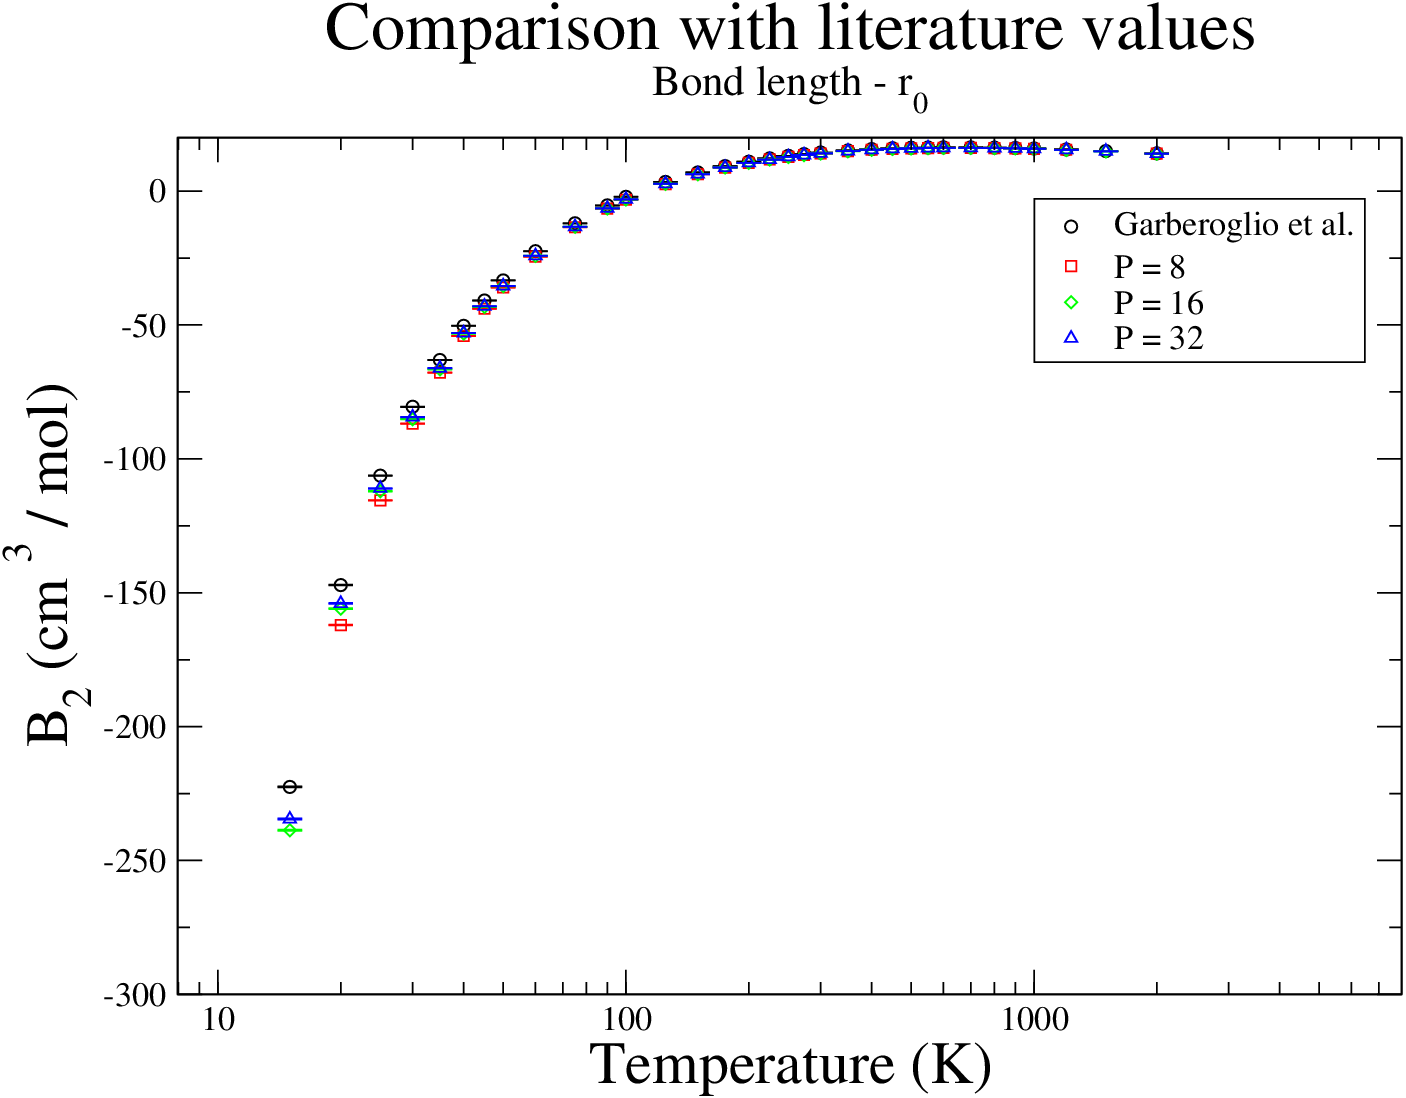
\includegraphics[scale=0.18,keepaspectratio]{8sfGResults.png}
	\end{figure}
	
	\end{frame}

	\begin{frame}
	\frametitle{Bond length \putCitation{Garberoglio2014}- $r_0$}
	\begin{figure}
	\centering
	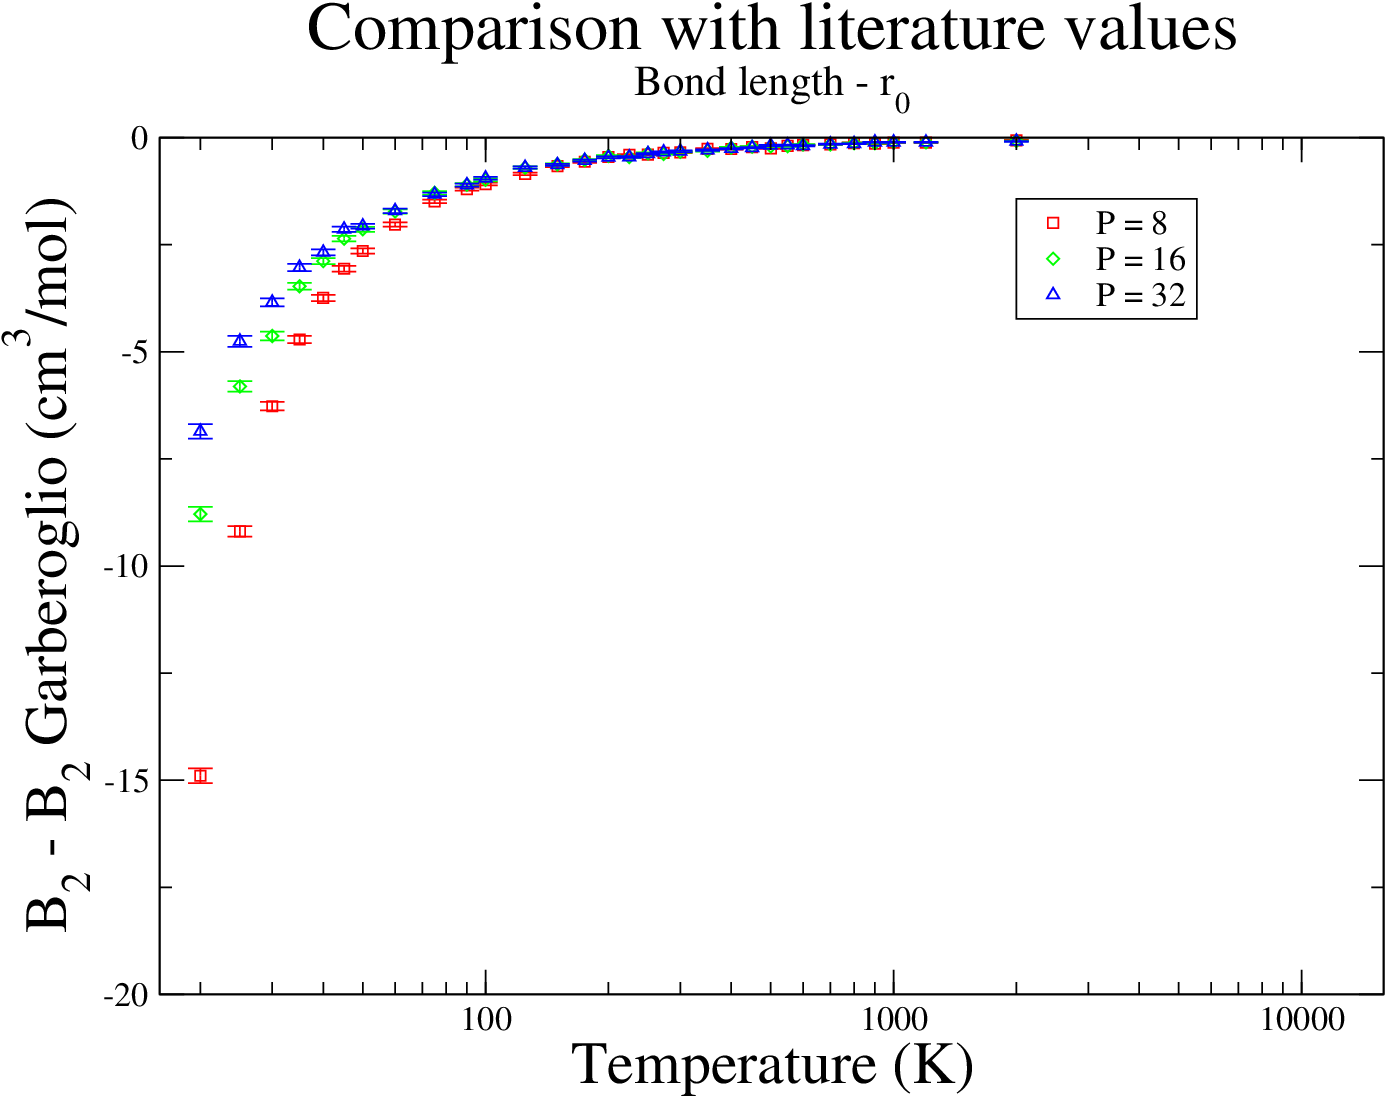
\includegraphics[scale=0.18,keepaspectratio]{8sfGResultsDiff.png}
	\end{figure}
	
	\end{frame}

	\begin{frame}
	\frametitle{Methods to handle flexibility}
	\begin{itemize}
	\justifying
	\item Instead of using ground state bond length ($r_0$) use average bond length at each temperature ($< r >_T$)
	\item Average the bond length values over internal degrees of freedom of each monomer, weighted by the appropriate wave function\putCitation{Garberoglio2012}
	\begin{equation*}
	<r>_T = \displaystyle\sum\limits_{n,J} p(n,J:T) < \chi_{nJ} | r | \chi_{nJ} >
	\end{equation*}
	\noindent where $n$ and $J$ are quantum numbers that define the vibrational and rotational state of $H_2$,respectively, while $\chi_{nJ}$ denotes the corresponding wave-function and \\
	\begin{equation*}
	p(n,J:T) = \frac{(2J + 1) \exp(-E(n,J)/T)}{\displaystyle\sum\limits_{n',J'} (2J' + 1) \exp(-E(n',J')/T)}
	\end{equation*}
	\noindent where $E(n',J')$ is the energy of the $(n',J')$ state
	\end{itemize}
	\end{frame}

	\begin{frame}
	\frametitle{Bond length\putCitation{Garberoglio2014}- $< r >_T$}
	\begin{figure}
	\centering
	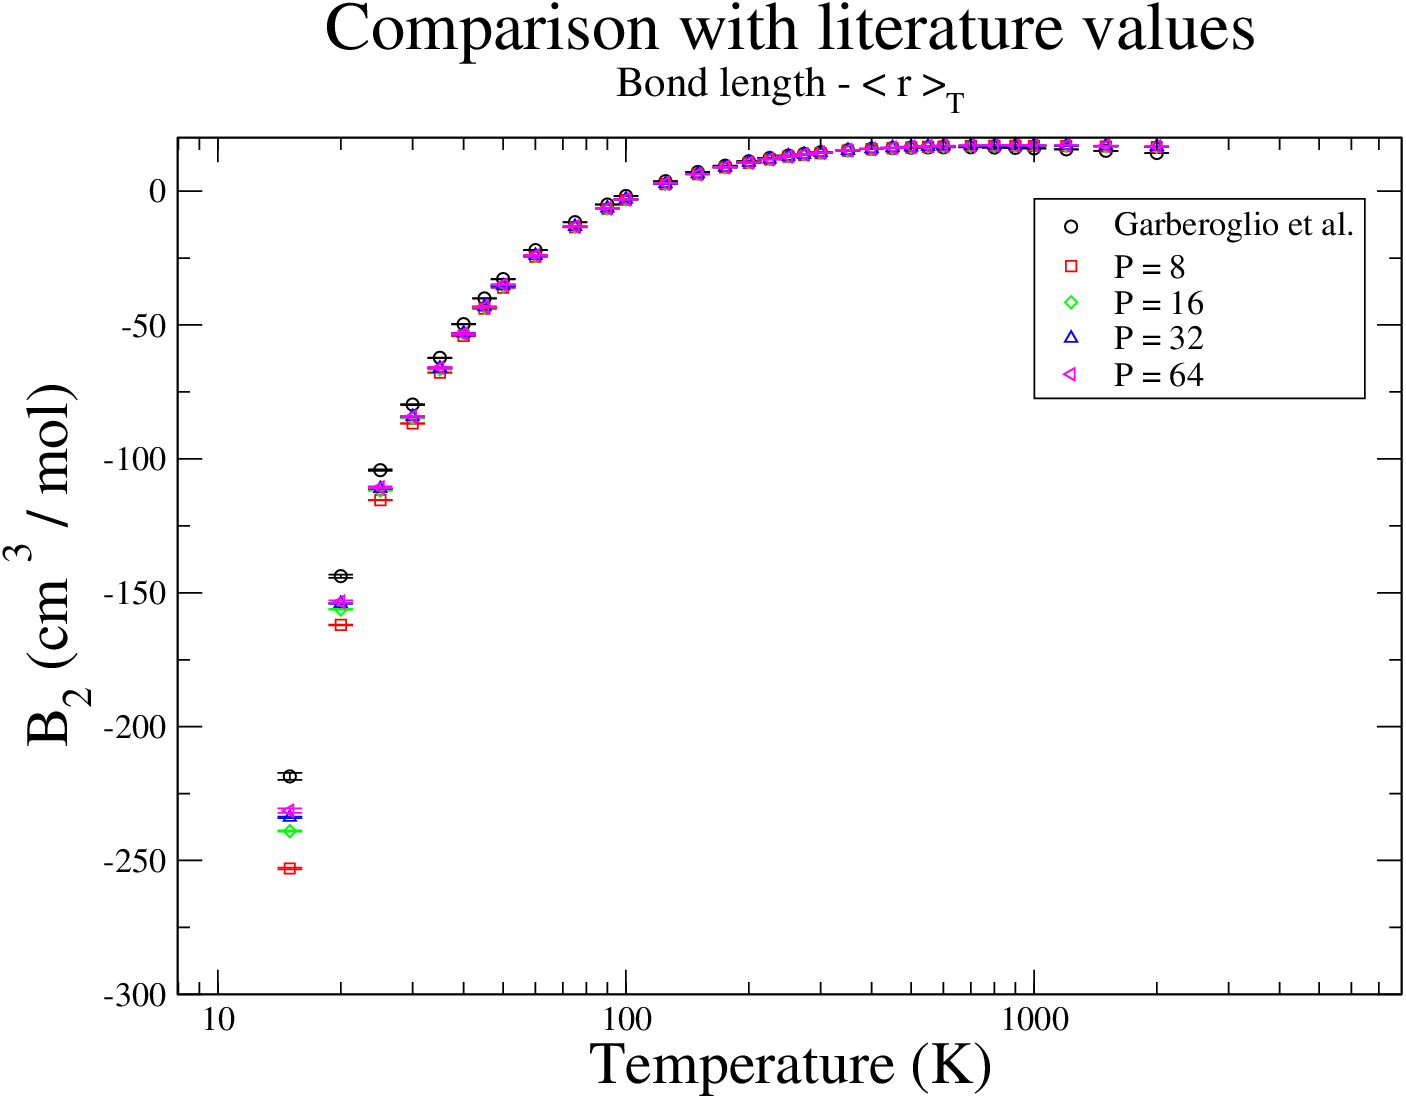
\includegraphics[scale=0.18,keepaspectratio]{8sfTAResults.png}
	\end{figure}
	
	\end{frame}

	\begin{frame}
	\frametitle{Bond length\putCitation{Garberoglio2014} - $< r >_T$}
	\begin{figure}
	\centering
	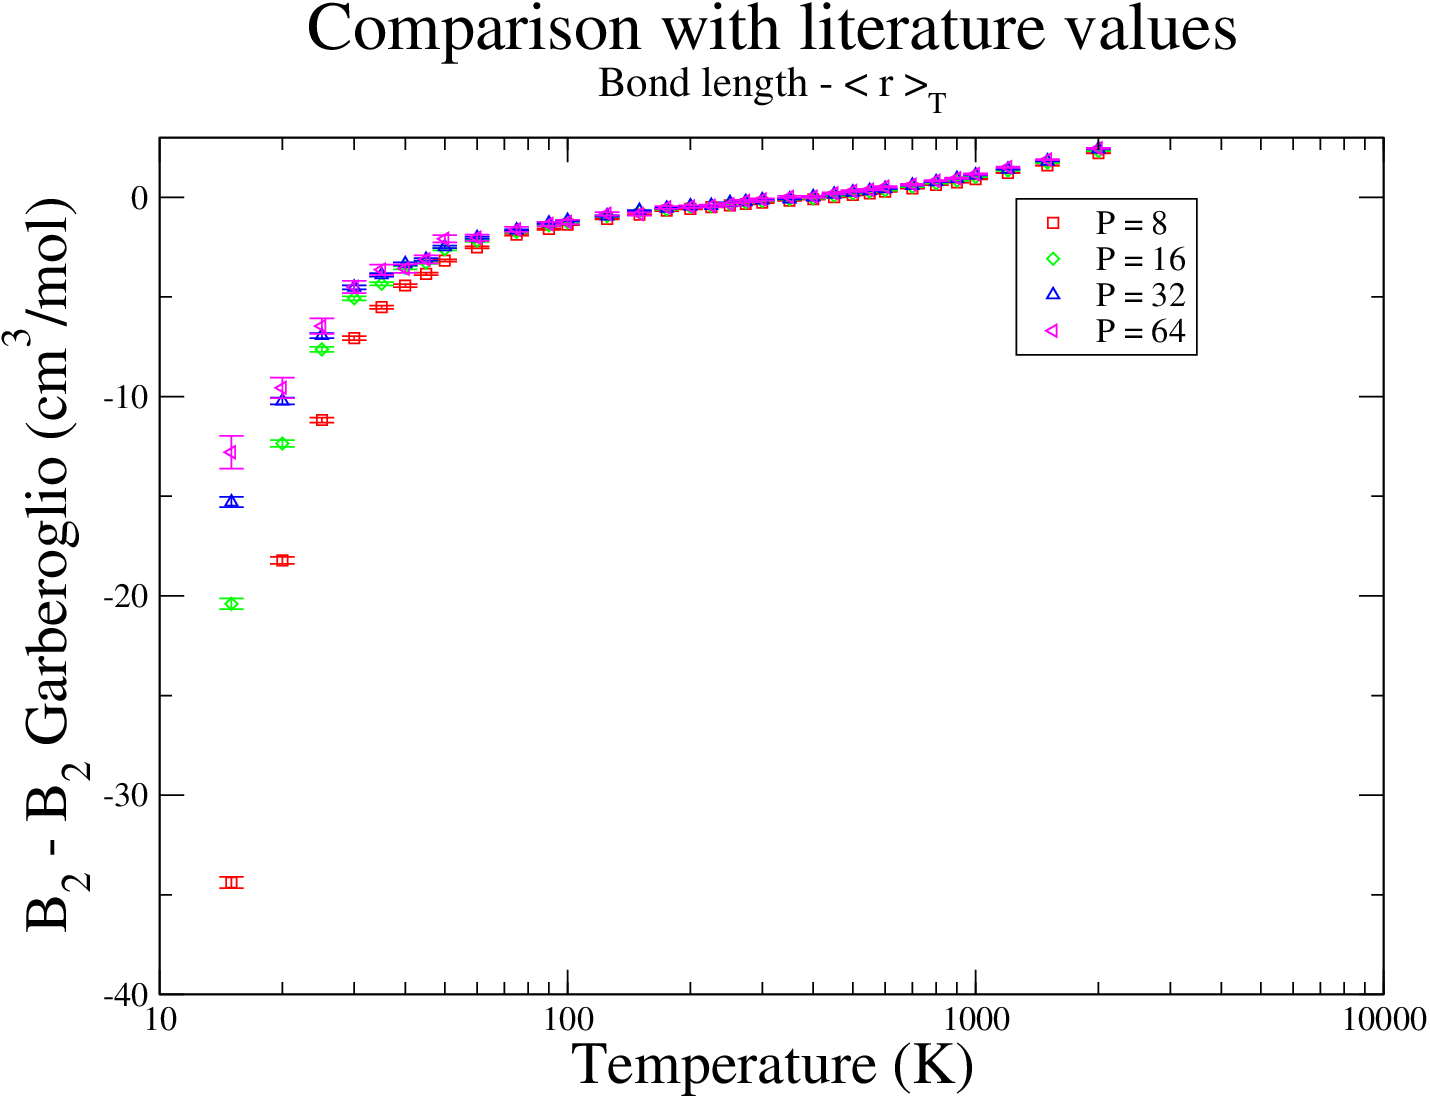
\includegraphics[scale=0.18,keepaspectratio]{8sfTAResultsDiff.png}
	\end{figure}
	
	\end{frame}

	\begin{frame}
	\frametitle{Bond length sampling - Introduction}
	\begin{itemize}
	\justifying
	\item Harmonic energy ($U_h$) of the springs and the intra-molecular potential energy ($U_i$) are the only two factors that affect the probability $\mathcal{P}$ of an image
	\item $U_h$ for adjacent monomers is given by:
	\begin{figure}
	\centering
	\def\svgscale{0.2}
	\input{uHarmonic.pdf_tex}
	\end{figure}
	\begin{equation*}
	\begin{aligned}
	U_h &= \frac{1}{2} \cdot k_h \cdot \displaystyle\sum\limits_{i=0}^P \Big( b_i^2 + b_j^2 - 2 \cdot b_i \cdot b_j \cdot \cos (\theta_{ij}) \Big)\\
	\text{where,} \: j &= i - 1 \: \text{for} \: i \ge 1 , j = P - 1\: \text{for} \: i = 0
	\end{aligned}
	\end{equation*}
	\item Intra-molecular potential that we use in our calculations is from Mielke et al.\putCitation{Mielke2002}
	\end{itemize}
	\end{frame}

	\begin{frame}
	\frametitle{$\mathcal{P}$ - actual probability of a configuration}
	\begin{itemize}
	\justifying
	\item Expression for $\mathcal{P}$ is almost exponential
	\item Consider the argument of the exponential
	\begin{equation*}
	- \log \mathcal{P} = \displaystyle\sum\limits_{i=0}^P \Bigg\{ k_h \cdot \Big( b_i^2 - b_i \cdot b_j \cdot \cos (\theta_{ij}) \Big) - 2 \cdot \log b_i + \frac{ \beta \cdot U_i (b_i)}{P} \Bigg\}
	\end{equation*}
	\item We can clearly see that it is not quadratic due to the presence of $U_i$
	\item Presence of cross terms such as $b_i \cdot b_j$ makes the bond lengths non-independent of each other
	\end{itemize}
	\end{frame}
	
	\begin{frame}
	\frametitle{Normal mode analysis}
	\begin{columns}[c]
	\begin{column}{6cm}
	\begin{itemize}
	\justifying
	\item Helps choose all bond lengths simultaneously
	\item Consider the combined behavior of all bond lengths as separate modes
	\item Construct matrix with second derivatives of $- \log \mathcal{P}$
	\item Compute eigenvalues $\lambda_i$ and eigenvectors $\vec{A_i}$ to separate out independent modes
	\item Evaluate new bond lengths simultaneously
	\end{itemize}
	\end{column}

	\begin{column}{4cm}
	\begin{figure}
	\centering
	\def\svgscale{0.3}
	\input{differentModes.pdf_tex}
	\end{figure}
	\end{column}
	\end{columns}
	\end{frame}

	\begin{frame}
	\frametitle{Bond length\putCitation{Garberoglio2014} - flexible}
	\begin{figure}
	\centering
	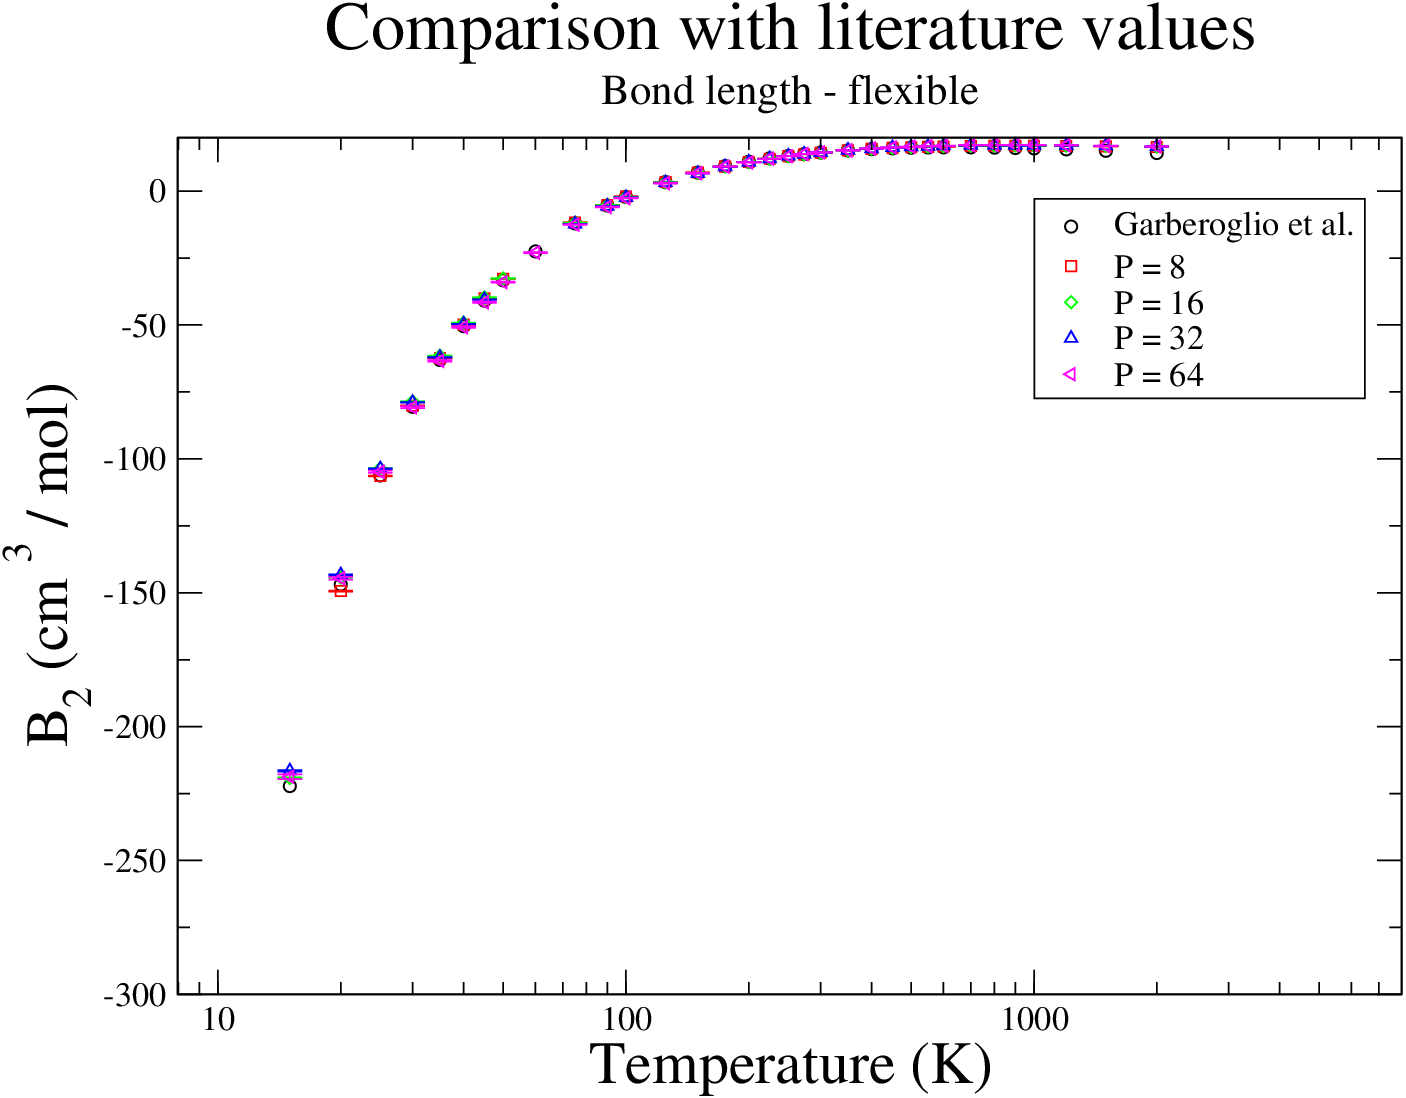
\includegraphics[scale=0.18,keepaspectratio]{8svBLResults.png}
	\end{figure}
	
	\end{frame}

	\begin{frame}
	\frametitle{Bond length\putCitation{Garberoglio2014} - flexible}
	\begin{figure}
	\centering
	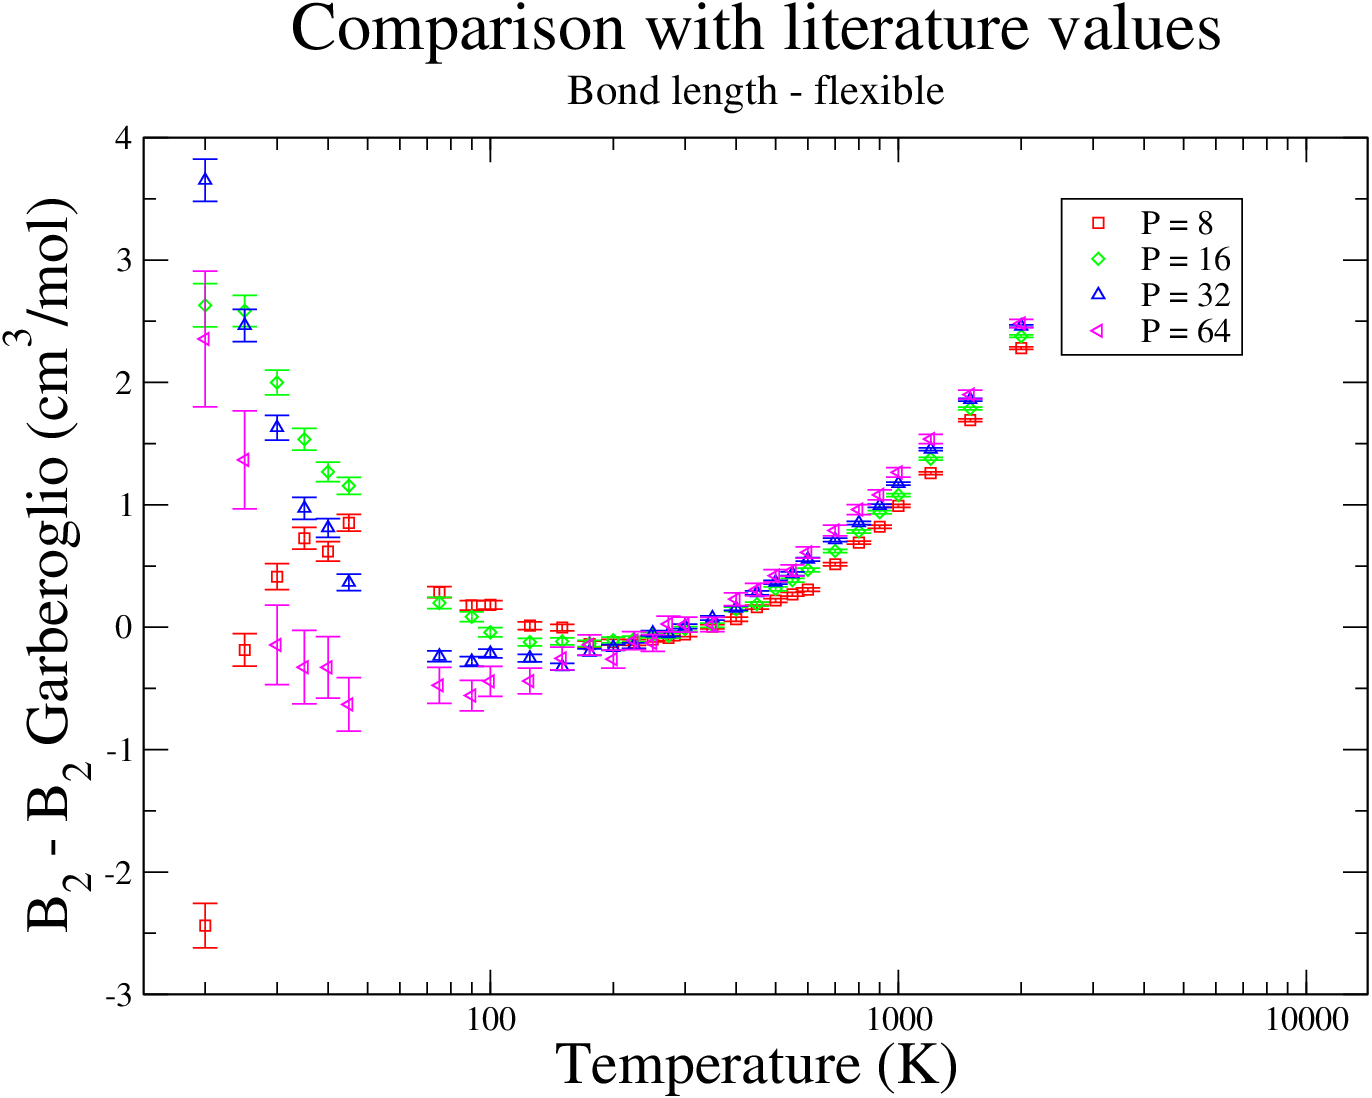
\includegraphics[scale=0.18,keepaspectratio]{8svBLResultsDiff.png}
	\end{figure}
	\end{frame}

	\begin{frame}
	\frametitle{Summary and future work}
	\begin{itemize}
	\justifying
	\item We have developed a bond length sampling algorithm that can be used to compute virial coefficients for flexible diatomic molecules
	\item We applied the algorithm for $H_2$ molecule and the resulting second virial coefficients are not in perfect agreement with literature data
	\item Fix remaining issues and improve efficiency of the move
	\item Apply the algorithm for other diatomic systems like $N_2$
	\item Extend the algorithm to other complicated systems like water
	\end{itemize}
	\end{frame}
	
	\begin{frame}
	\setbeamertemplate{headline}{}
	\frametitle{Acknowledgment}
	\begin{itemize}
	\item My advisor Dr. David Kofke
	\item Dr. Andrew Schultz
	\item Members of the Kofke group
	\item Funding:
	\begin{figure}
	\centering
	
\includegraphics[width=5cm,keepaspectratio]{nsfLogo.png}
	\end{figure}
	\item Computational resources:
	\begin{figure}
	
\includegraphics[width=5cm,keepaspectratio]{ccrLogo.jpg}
	\end{figure}
	\item We would like to thank Dr. Allan H. Harvey for insightful discussions
	\end {itemize}
	\end{frame}

	\begin{frame}
	\frametitle{Thank you for your attention!}
	\begin{center}
	\huge{Questions???}
	\end{center}
	\end{frame}

	\begin{frame}
	\frametitle{$P_{act}$}
	\begin{itemize}
	\item Let $P_{act} = \exp (-z_{act})$ where $z_{act}$ can be defined as follows:-
	\begin{equation*} \label {zact}
	z_{act} = \displaystyle\sum\limits_{i=0}^P \Bigg\{ k_h \cdot \Big( b_i^2 - b_i \cdot b_j \cdot \cos (\theta_{ij}) \Big) - 2 \cdot \log b_i + \frac{ \beta \cdot U_i (b_i)}{P} \Bigg\}
	\end{equation*}
	\item Since $z_{act}$ is not quadratic, it is not easy to sample from
	\item All bond lengths not independent of each other
	\end{itemize}
	\end{frame}

	\begin{frame}
	\frametitle{Assumptions and modifications}
	\begin{itemize}
	\justifying
	\item $z_{act}$ is given by:
	\begin{equation*}
	z_{act} = \displaystyle\sum\limits_{i=0}^P \Bigg\{ k_h \cdot \Big( b_i^2 - b_i \cdot b_j \cdot \cos (\theta_{ij}) \Big) - 2 \cdot \log b_i + \frac{ \beta \cdot U_i (b_i)}{P} \Bigg\}
	\end{equation*}
	\item Finding $b_{min}$, given as the solution of $\frac{\partial z_{act}}{\partial b_i} \Big|_{b_i = b_{min}} = 0$, before each move can be very inefficient
	\item Let $z_{act}^*$ be given by:
	\begin{equation*}
	z_{act}^* = \displaystyle\sum\limits_{i=0}^P \Bigg\{ k_h \cdot \Big( b_i^2 - b_i \cdot b_j \Big) - \frac{2 \cdot \log b_i}{P} + \frac{ \beta \cdot U_i (b_i)}{P} \Bigg\}
	\end{equation*}
	\item Find $b_{min}$ using $\frac{\partial z_{act}^*}{\partial b_i} \Big|_{b_i = b_{min}} = 0$, set $\displaystyle\frac{\partial z_{act}}{\partial b_i} = \displaystyle\frac{\partial z_{act}^*}{\partial b_i}$ and solve for $\theta_{ij}$
	\end{itemize}
	\end{frame}

	\begin{frame}
	\frametitle{Assumptions and modifications}
	\begin{itemize}
	\item Let $\frac{\partial z_{act}}{\partial b_i} = \frac{\partial z_{act}^*}{\partial b_i}$ solve for $\cos (\theta_{ij})$
	\item $\cos (\theta_{ij}) = 1 - \frac{P-1}{P \cdot k_h \cdot b_i^2}$
	\item Compute $b_{min}$ using $\frac{\partial z_{act}}{\partial b_i} \Bigg|_{b_i = b_{min}} = \frac{\partial z_{act}^*}{\partial b_i} \Bigg|_{b_i = b_{min}} = 0$
	\end{itemize}
	\end{frame}

	\begin{frame}
	\frametitle{Conclusions}
	\begin{itemize}
	\item Let $\frac{\partial z_{act}}{\partial b_i} = \frac{\partial z_{act}^*}{\partial b_i}$ solve for $\cos (\theta_{ij})$
	\item $\cos (\theta_{ij}) = 1 - \frac{P-1}{P \cdot k_h \cdot b_i^2}$
	\item Compute $b_{min}$ using $\frac{\partial z_{act}}{\partial b_i} \Bigg|_{b_i = b_{min}} = \frac{\partial z_{act}^*}{\partial b_i} \Bigg|_{b_i = b_{min}} = 0$
	\end{itemize}
	\end{frame}

	\begin{frame}
	\frametitle{Future work}
	\begin{itemize}
	\item Let $\frac{\partial z_{act}}{\partial b_i} = \frac{\partial z_{act}^*}{\partial b_i}$ solve for $\cos (\theta_{ij})$
	\item $\cos (\theta_{ij}) = 1 - \frac{P-1}{P \cdot k_h \cdot b_i^2}$
	\item Compute $b_{min}$ using $\frac{\partial z_{act}}{\partial b_i} \Bigg|_{b_i = b_{min}} = \frac{\partial z_{act}^*}{\partial b_i} \Bigg|_{b_i = b_{min}} = 0$
	\end{itemize}
	\end{frame}

	\begin{frame}
	\frametitle{Future work}
	\begin{itemize}
	\item Let $\frac{\partial z_{act}}{\partial b_i} = \frac{\partial z_{act}^*}{\partial b_i}$ solve for $\cos (\theta_{ij})$
	\item $\cos (\theta_{ij}) = 1 - \frac{P-1}{P \cdot k_h \cdot b_i^2}$
	\item Compute $b_{min}$ using $\frac{\partial z_{act}}{\partial b_i} \Bigg|_{b_i = b_{min}} = \frac{\partial z_{act}^*}{\partial b_i} \Bigg|_{b_i = b_{min}} = 0$
	\end{itemize}
	\end{frame}
	
\end{document}
